\documentclass{report}
%%%%%%%%%%%%%% preamble.tex %%%%%%%%%%%%%%
\usepackage[T1]{fontenc}
\usepackage{etoolbox}
% Page Setup
\usepackage[letterpaper, tmargin=2cm, rmargin=0.5in, lmargin=0.5in, bmargin=80pt, footskip=.2in]{geometry}
\usepackage{adjustbox}
\usepackage{graphicx}
\usepackage{tikz}
\usepackage{mathrsfs}
\usepackage{mdframed}

% Create a new toggle
\newtoggle{firstsection}

% Redefine the \chapter command to reset the toggle for each new chapter
\let\oldchapter\chapter
\renewcommand{\chapter}{\toggletrue{firstsection}\oldchapter}

% Redefine the \section command to check the toggle
\let\oldsection\section
\renewcommand{\section}{
    \iftoggle{firstsection}
    {\togglefalse{firstsection}} % If it's the first section, just switch off the toggle for next sections
    {\clearpage} % If it's not the first section, start a new page
    \oldsection
}

% Abstract Design

\usepackage{lipsum}

\renewenvironment{abstract}
 {% Start of environment
  \quotation
  \small
  \noindent
  \rule{\linewidth}{.5pt} % Draw the rule to match the linewidth
  \par\smallskip
  {\centering\bfseries\abstractname\par}\medskip
 }
 {% End of environment
  \par\noindent
  \rule{\linewidth}{.5pt} % Ensure the closing rule also matches
  \endquotation
 }

% Mathematics
\usepackage{amsmath,amsfonts,amsthm,amssymb,mathtools}
\usepackage{xfrac}
\usepackage[makeroom]{cancel}
\usepackage{enumitem}
\usepackage{nameref}
\usepackage{multicol,array}
\usepackage{tikz-cd}
\usepackage{array}
\usepackage{multirow}% http://ctan.org/pkg/multirow
\usepackage{graphicx}

% Colors
\usepackage[dvipsnames]{xcolor}
\definecolor{myg}{RGB}{56, 140, 70}
\definecolor{myb}{RGB}{45, 111, 177}
\definecolor{myr}{RGB}{199, 68, 64}
% Define more colors here...
\definecolor{olive}{HTML}{6B8E23}
\definecolor{orange}{HTML}{CC5500}
\definecolor{brown}{HTML}{8B4513}
% Hyperlinks
\usepackage{bookmark}
\usepackage[colorlinks=true,linkcolor=blue,urlcolor=blue,citecolor=blue,anchorcolor=blue]{hyperref}
\usepackage{xcolor}
\hypersetup{
    colorlinks,
    linkcolor={red!50!black},
    citecolor={blue!50!black},
    urlcolor={blue!80!black}
}

% Text-related
\usepackage{blindtext}
\usepackage{fontsize}
\changefontsize[14]{14}
\setlength{\parindent}{0pt}
\linespread{1.2}

% Theorems and Definitions
\usepackage{amsthm}
\renewcommand\qedsymbol{$\blacksquare$}

% Define a new theorem style
\newtheoremstyle{mytheoremstyle}% name
  {}% Space above
  {}% Space below
  {}% Body font
  {}% Indent amount
  {\bfseries}% Theorem head font
  {.}% Punctuation after theorem head
  {.5em}% Space after theorem head
  {}% Theorem head spec (can be left empty, meaning ‘normal’)

% Apply the new theorem style to theorem-like environments
\theoremstyle{mytheoremstyle}

\newtheorem{theorem}{Theorem}[section]  
\newtheorem{definition}[theorem]{Definition} 
\newtheorem{lemma}[theorem]{Lemma}  
\newtheorem{corollary}[theorem]{Corollary}
\newtheorem{axiom}[theorem]{Axiom}
\newtheorem{example}[theorem]{Example}
\newtheorem{equiv_def}[theorem]{Equivalent Definition}

% tcolorbox Setup
\usepackage[most,many,breakable]{tcolorbox}
\tcbuselibrary{theorems}

% Define custom tcolorbox environments here...

%================================
% EXAMPLE BOX
%================================
% After you have defined the style and other theorem environments
\definecolor{myexamplebg}{RGB}{245, 245, 245} % Very light grey for background
\definecolor{myexamplefr}{RGB}{120, 120, 120} % Medium grey for frame
\definecolor{myexampleti}{RGB}{60, 60, 60}    % Darker grey for title

\newtcbtheorem[]{Example}{Example}{
    colback=myexamplebg,
    breakable,
    colframe=myexamplefr,
    coltitle=myexampleti,
    boxrule=1pt,
    sharp corners,
    detach title,
    before upper=\tcbtitle\par\vspace{-20pt}, % Reduced the space after the title
    fonttitle=\bfseries,
    description font=\mdseries,
    separator sign none,
    description delimiters={}{}, % No delimiters around the title
}{ex}
%================================
% Solution BOX
%================================
\makeatletter
\newtcolorbox{solution}{enhanced,
	breakable,
	colback=white,
	colframe=myg!80!black,
	attach boxed title to top left={yshift*=-\tcboxedtitleheight},
	title=Solution,
	boxed title size=title,
	boxed title style={%
			sharp corners,
			rounded corners=northwest,
			colback=tcbcolframe,
			boxrule=0pt,
		},
	underlay boxed title={%
			\path[fill=tcbcolframe] (title.south west)--(title.south east)
			to[out=0, in=180] ([xshift=5mm]title.east)--
			(title.center-|frame.east)
			[rounded corners=\kvtcb@arc] |-
			(frame.north) -| cycle;
		},
}
\makeatother

% %================================
% % Question BOX
% %================================
\makeatletter
\newtcbtheorem{question}{Question}{enhanced,
	breakable,
	colback=white,
	colframe=myb!80!black,
	attach boxed title to top left={yshift*=-\tcboxedtitleheight},
	fonttitle=\bfseries,
	title={#2},
	boxed title size=title,
	boxed title style={%
			sharp corners,
			rounded corners=northwest,
			colback=tcbcolframe,
			boxrule=0pt,
		},
	underlay boxed title={%
			\path[fill=tcbcolframe] (title.south west)--(title.south east)
			to[out=0, in=180] ([xshift=5mm]title.east)--
			(title.center-|frame.east)
			[rounded corners=\kvtcb@arc] |-
			(frame.north) -| cycle;
		},
	#1
}{question}
\makeatother

%%%%%%%%%%%%%%%%%%%%%%%%%%%%%%%%%%%%%%%%%%%
% TABLE OF CONTENTS
%%%%%%%%%%%%%%%%%%%%%%%%%%%%%%%%%%%%%%%%%%%


\usepackage{tikz}
\definecolor{doc}{RGB}{0,60,110}
\usepackage{titletoc}
\contentsmargin{0cm}
\titlecontents{chapter}[14pc]
{\addvspace{30pt}%
	\begin{tikzpicture}[remember picture, overlay]%
		\draw[fill=doc!60,draw=doc!60] (-7,-.1) rectangle (-0.9,.5);%
		\pgftext[left,x=-5.5cm,y=0.2cm]{\color{white}\Large\sc\bfseries Chapter\ \thecontentslabel};%
	\end{tikzpicture}\color{doc!60}\large\sc\bfseries}%
{}
{}
{\;\titlerule\;\large\sc\bfseries Page \thecontentspage
	\begin{tikzpicture}[remember picture, overlay]
		\draw[fill=doc!60,draw=doc!60] (2pt,0) rectangle (4,0.1pt);
	\end{tikzpicture}}%
\titlecontents{section}[3.7pc]
{\addvspace{2pt}}
{\contentslabel[\thecontentslabel]{3pc}}
{}
{\hfill\small \thecontentspage}
[]
\titlecontents*{subsection}[3.7pc]
{\addvspace{-1pt}\small}
{}
{}
{\ --- \small\thecontentspage}
[ \textbullet\ ][]

\makeatletter
\renewcommand{\tableofcontents}{
	\chapter*{%
	  \vspace*{-20\p@}%
	  \begin{tikzpicture}[remember picture, overlay]%
		  \pgftext[right,x=15cm,y=0.2cm]{\color{doc!60}\Huge\sc\bfseries \contentsname};%
		  \draw[fill=doc!60,draw=doc!60] (13,-.75) rectangle (20,1);%
		  \clip (13,-.75) rectangle (20,1);
		  \pgftext[right,x=15cm,y=0.2cm]{\color{white}\Huge\sc\bfseries \contentsname};%
	  \end{tikzpicture}}%
	\@starttoc{toc}}
\makeatother

\newcommand{\liff}{\llap{$\iff$}}
\newcommand{\rap}[1]{\rrap{\text{ (#1)}}}
\newcommand{\red}[1]{\textcolor{red}{#1}}
\newcommand{\blue}[1]{\textcolor{blue}{#1}}
\newcommand{\vi}[1]{\textcolor{violet}{#1}}
\newcommand{\olive}[1]{\textcolor{olive}{#1}}
\newcommand{\teal}[1]{\textcolor{teal}{#1}}
\newcommand{\brown}[1]{\textcolor{brown}{#1}}
\newcommand{\orange}[1]{\textcolor{orange}{#1}}
\newcommand{\tCaC}{\text{ \CaC }}
\newcommand{\CaC}{\red{CaC} }
\newcommand{\As}[1]{Assume \red{#1}}
\newcommand{\vdone}{\vi{\text{ (done) }}}
\newcommand{\bdone}{\blue{\text{ (done) }}}
\newcommand{\tdone}{\teal{\text{ (done) }}}
\newcommand{\odone}{\olive{\text{ (done) }}}
\newcommand{\bodone}{\brown{\text{ (done) }}}
\newcommand{\ordone}{\orange{\text{ (done) }}}
\newcommand{\ld}{\lambda}
\newcommand{\vecta}[1]{\textbf{#1}}
\newcommand{\set}[1]{\left\{ #1 \right\}}
\newcommand{\bset}[1]{\Big\{ #1 \Big\}}
\newcommand{\inR}{\in\R}
\newcommand{\inn}{\in\N}
\newcommand{\inz}{\in\Z}
\newcommand{\inr}{\in\R}
\newcommand{\inc}{\in\C}
\newcommand{\inq}{\in\Q}
\newcommand{\norm}[1]{\| #1 \|}
\newcommand{\bnorm}[1]{\Big\| #1 \Big\|}
\newcommand{\gen}[1]{\langle #1 \rangle}
\newcommand{\abso}[1]{\left|#1\right|}
\newcommand{\myref}[2]{\hyperref[#2]{#1\ \ref*{#2}}}
\newcommand{\customref}[2]{\hyperref[#1]{#2}}
\newcommand{\power}[1]{\mathcal{P}(#1)}
\newcommand{\dcup}{\mathbin{\dot{\cup}}}
\newcommand{\diam}[1]{\text{diam}\, #1}
\newcommand{\at}{\Big|}
\newcommand{\quotient}{\diagup}
\let\originalphi\phi % Store the original \phi in \originalphi
\renewcommand{\phi}{\varphi} % Redefine \phi to \varphi
\newcommand{\pfi}{\originalphi} % Define \pfi to display the original \phi
\newcommand{\diota}{\dot{\iota}}
\newcommand{\Log}{\operatorname{Log}}
\newcommand{\id}{\text{\textbf{id}}}
\usepackage{amsmath}

\makeatletter
\NewDocumentCommand{\extp}{e{^}}{%
  \mathop{\mathpalette\extp@{#1}}\nolimits
}
\NewDocumentCommand{\extp@}{mm}{%
  \bigwedge\nolimits\IfValueT{#2}{^{\extp@@{#1}#2}}%
  \IfValueT{#1}{\kern-2\scriptspace\nonscript\kern2\scriptspace}%
}
\newcommand{\extp@@}[1]{%
  \mkern
    \ifx#1\displaystyle-1.8\else
    \ifx#1\textstyle-1\else
    \ifx#1\scriptstyle-1\else
    -0.5\fi\fi\fi
  \thinmuskip
}
\makeatletter
\usepackage{pifont}
\makeatletter
\newcommand\Pimathsymbol[3][\mathord]{%
  #1{\@Pimathsymbol{#2}{#3}}}
\def\@Pimathsymbol#1#2{\mathchoice
  {\@Pim@thsymbol{#1}{#2}\tf@size}
  {\@Pim@thsymbol{#1}{#2}\tf@size}
  {\@Pim@thsymbol{#1}{#2}\sf@size}
  {\@Pim@thsymbol{#1}{#2}\ssf@size}}
\def\@Pim@thsymbol#1#2#3{%
  \mbox{\fontsize{#3}{#3}\Pisymbol{#1}{#2}}}
\makeatother
% the next two lines are needed to avoid LaTeX substituting upright from another font
\input{utxmia.fd}
\DeclareFontShape{U}{txmia}{m}{n}{<->ssub * txmia/m/it}{}
% you may also want
\DeclareFontShape{U}{txmia}{bx}{n}{<->ssub * txmia/bx/it}{}
% just in case
%\DeclareFontShape{U}{txmia}{l}{n}{<->ssub * txmia/l/it}{}
%\DeclareFontShape{U}{txmia}{b}{n}{<->ssub * txmia/b/it}{}
% plus info from Alan Munn at https://tex.stackexchange.com/questions/290165/how-do-i-get-a-nicer-lambda?noredirect=1#comment702120_290165
\newcommand{\pilambdaup}{\Pimathsymbol[\mathord]{txmia}{21}}
\renewcommand{\lambda}{\pilambdaup}
\renewcommand{\tilde}{\widetilde}
\DeclareMathOperator*{\esssup}{ess\,sup}
\newcommand{\bluecheck}{}%
\DeclareRobustCommand{\bluecheck}{%
  \tikz\fill[scale=0.4, color=blue]
  (0,.35) -- (.25,0) -- (1,.7) -- (.25,.15) -- cycle;%
}


\usepackage{tikz}
\newcommand*{\DashedArrow}[1][]{\mathbin{\tikz [baseline=-0.25ex,-latex, dashed,#1] \draw [#1] (0pt,0.5ex) -- (1.3em,0.5ex);}}

\newcommand{\C}{\mathbb{C}}	
\newcommand{\F}{\mathbb{F}}
\newcommand{\N}{\mathbb{N}}
\newcommand{\Q}{\mathbb{Q}}
\newcommand{\R}{\mathbb{R}}
\newcommand{\Z}{\mathbb{Z}}



\title{\Huge{HWs}}
\author{\huge{Eric Liu}}
\date{}
\begin{document}
\maketitle
\newpage% or \cleardoublepage
% \pdfbookmark[<level>]{<title>}{<dest>}
\pdfbookmark[section]{\contentsname}{toc}
\tableofcontents
\pagebreak

\chapter{General Analysis HW}
\section{HW1}
\begin{question}{}{}
Show $\R^n$ is complete.
\end{question}
\begin{proof}
Let $\textbf{x}_k$ be an arbitrary Cauchy sequence in $\R^n$. We are required to show  $\textbf{x}_k$ converge in $\R^n$. For each $k$, denote  $\textbf{x}_k$ by $(x_{(1,k)},\dots ,x_{(n,k)})$. We claim that for each $i \in \set{1,\dots ,n}$
\begin{align*}
x_{(i,k)}\text{ is a Cauchy sequence }
\end{align*}
Fix $i$ and $\epsilon >0$. To show $x_{(i,k)}$ is a Cauchy sequence, we are required to find $N\inn$ such that for all $r,m\geq N$ we have 
\begin{align*}
\abso{x_{(i,r)}-x_{(i,m)}}\leq \epsilon 
\end{align*}
Because $\textbf{x}_k$ is a Cauchy sequence in $\R^n$, we know there exists  $N\inn$ such that for all $r,m\geq N$, we have 
\begin{align*}
\abso{\textbf{x}_r-\textbf{x}_m}< \epsilon 
\end{align*}
Fix such $N$ and arbitrary $r,m\geq M$. Observe 
\begin{align*}
\abso{x_{(i,r)}-x_{(i,m)}}\leq \sqrt{\sum_{j=1}^n \abso{x_{(j,r)}-x_{(j,m)}}^2}= \abso{\textbf{x}_r - \textbf{x}_m}< \epsilon 
\end{align*}
We have proved that for each $i\in \set{1,\dots ,n}$, the real sequence $x_{(i,k)}$ is Cauchy. We now claim that for each $i \in \set{1,\dots, n}$, we have 
\begin{align*}
  \limsup_{r\to\infty} x_{(i,r)}\inr \text{ and }\lim_{k\to \infty}x_{(i,k)}= \limsup_{r\to\infty} x_{(i,r)}
\end{align*}
Again fix $i$. Because $x_{(i,k)}$ is a Cauchy sequence, we know there exists some $N$ such that for all $r,m\geq N$, we have 
 \begin{align*}
\abso{x_{(i,r)}-x_{(i,m)}}<1
\end{align*}
This implies that for all $r\geq N$, we have 
\begin{align}
x_{(i,r)}< x_{(i,N)}+1 \label{ran1}
\end{align}
\myref{Equation}{ran1} then tell us 
\begin{align*}
x_{(i,N)}+1\text{ is an upper bound of }\set{x_{(i,r)}:r\geq N}
\end{align*}
Then by definition of $\sup $, we have
\begin{align*}
\sup \set{x_{(i,r)}:r\geq N} \leq x_{(i,N)}+1 \inr
\end{align*}
This then implies $\limsup_{r\to\infty} x_{(i,r)}\inr$. We now prove 
\begin{align}
\label{ran2}
\lim_{k\to \infty}x_{(i,k)}= \limsup_{r\to\infty} x_{(i,r)}
\end{align}
Fix $\epsilon >0$. We are required to find $N$ such that
\begin{align*}
\forall k\geq N, \abso{x_{(i,k)}-\limsup_{r\to\infty}x_{(i,r)}} \leq \epsilon 
\end{align*}
Because $\set{x_{(i,k)}}_{k\inn}$ is a Cauchy sequence, we can let $N_0$ satisfy 
\begin{align*}
\forall k,m\geq N_0, \abso{x_{(i,k)}-x_{(i,m)}}<\frac{\epsilon}{2}
\end{align*}
Because $\sup \set{x_{(i,k)}:k\geq N'}\searrow \limsup_{r\to\infty} x_{(i,r)}$ as $N'\to \infty$, we know there exists $N_1>N_0$ such that 
 \begin{align*}
\limsup_{r\to\infty} x_{(i,r)}-\frac{\epsilon}{2} <\sup \set{x_{(i,k)}:k\geq N_0}\leq \limsup_{r\to\infty}  x_{(i,r)} + \frac{\epsilon}{2} 
\end{align*}
Then because $\limsup_{r\to\infty} x_{(i,r)}-\frac{\epsilon}{2}$ is strictly smaller than the smallest upper bound of $\set{x_{(i,k)}:k\geq N_1}$, we see $\limsup_{n\to\infty} x_{(i,r)}-\frac{\epsilon}{2}$ is not an upper bound of $\set{x_{(i,k)}:k\geq N_1}$. This implies the existence of some $N$ such that  $N\geq N_1$ and
\begin{align*}
\limsup_{r\to\infty} x_{(i,r)}-\frac{\epsilon}{2}< x_{(i,N)}\leq \limsup_{r\to\infty}x_{(i,r)} + \frac{\epsilon}{2}
\end{align*}
Now observe that for all $k\geq N$, because $N\geq N_1\geq N_0$ 
\begin{align*}
  \limsup_{r\to\infty} x_{(i,r)} - \epsilon <x_{(i,N)}-\frac{\epsilon}{2}<x_{(i,k)}< x_{(i,N)}+\frac{\epsilon}{2} \leq \limsup_{r\to\infty} x_{(i,r)} + \epsilon   
\end{align*}
This implies for all $k\geq N$, we have 
\begin{align*}
\abso{x_{(i,k)}-\limsup_{r\to\infty} x_{(i,r)}}\leq \epsilon 
\end{align*}
We have just proved \myref{Equation}{ran2}. Lastly, to close out the proof, we show 
\begin{align}
\label{ran3}
\lim_{k\to \infty}\textbf{x}_k = \Big(\lim_{k\to \infty}x_{(1,k)},\dots ,\lim_{k\to \infty}x_{(n,k)}\Big)
\end{align}
Fix $\epsilon >0$. For each $i \in \set{1,\dots ,n}$, let $N_i$ satisfy 
 \begin{align*}
  \forall r\geq N_i ,\abso{x_{(i,r)}- \lim_{k\to \infty}x_{(i,k)}}\leq  \frac{\epsilon }{\sqrt{n} }
\end{align*}
Observe that for all $r\geq \max_{i\in \set{1,\dots,n}} N_i$, we have 
\begin{align*}
\abso{\textbf{x}_r - \Big(\lim_{k\to \infty}x_{(1,k)},\dots ,\lim_{k\to \infty}x_{(n,k)} \Big)}&=\sqrt{\sum_{i=1}^n \abso{x_{(i,r)}- \lim_{k\to \infty}x_{(i,k)}}^2} \\
&\leq \sqrt{\sum_{i=1}^n \frac{\epsilon^2}{n}}=\epsilon 
\end{align*}
We have proved \myref{Equation}{ran3}.











\end{proof}
\begin{question}{}{}
Show $\Q$ is dense in $\R$. 
\end{question}
\begin{proof}
Fix $x\inr$ and $\epsilon >0$. To show $\Q$ is dense in  $\R$, we have to find $q\inq$ such that $\abso{x-q}<\epsilon $.\\

Let $m\inn$ satisfy $\frac{1}{m}<\epsilon $. Let $n$ be the largest integer such that $n\leq mx$. Because $n$ is the largest integer such that $n\leq mx$, we know $mx-n<1$, otherwise we can deduce $n+1\leq mx$, which is impossible, since $n+1$ is an integer and $n$ is the largest integer such that $n\leq mx$. We now see that 
\begin{align*}
\frac{n}{m}\inq \text{ and }\abso{x-\frac{n}{m}}=\frac{mx-n}{m}< \frac{1}{m}<\epsilon 
\end{align*}



\end{proof}
\begin{theorem}
\textbf{(Distance Formula)} Given two subsets $A,B$ of a metric space, we have 
\begin{align*}
d(A,B)= \inf_{b \in B}d(A,b)
\end{align*}
\end{theorem}
\begin{proof}
Fix arbitrary $b \in B$. It is clear that 
\begin{align*}
d(A,B)\leq d(A,b)
\end{align*}
It then follows $d(A,B)\leq \inf_{b \in B}d(A,b)$. Fix arbitrary $a \in A$ and $b_0 \in B$. Observe that 
\begin{align*}
d(a,b_0)\geq  d(A,b_0) \geq \inf_{b \in B}d(A,b)
\end{align*}
It then follows $\inf_{b \in B}d(A,b)\leq d(A,B)$. 
\end{proof}
\begin{question}{}{}
Let $E_1,E_2$ be non-empty sets in  $\R^n$ with $E_1$ closed and  $E_2$ compact. Show that there are points  $x_1\in E_1$ and $x_2 \in E_2$ such that 
\begin{align*}
d(E_1,E_2)=\abso{x_1-x_2}
\end{align*}
Deduce that $d(E_1,E_2)$ is positive if such $E_1,E_2$ are disjoint. 
\end{question}

\begin{proof}
Because 
\begin{enumerate}[label=(\alph*)]
  \item $f(x)\triangleq d (E_1,x)$ is a continuous function on $\R^n$. 
  \item $E_2$ is compact. 
\end{enumerate}
It now follows by EVT there exists some  $x_2 \in E_2$ such that 
\begin{align*}
d(E_1,x_2)=\min_{x \in E_2} d(E_1,x)=\inf_{x \in E_2}d(E_1,x)=d(E_1,E_2)
\end{align*}
where the last equality is proved above. We can now reduce the problem into finding $x_1$ in $E_1$ such that  
\begin{align*}
  \vi{d(x_1,x_2)=d(E_1,x_2)}
\end{align*}
For each $n\inn$, let $t_n$ satisfy 
 \begin{align*}
t_n \in E_1\text{ and }d(t_n,x_2)< d(E_1,x_2) + \frac{1}{n}
\end{align*}
Clearly, $t_n$ is a bounded sequence. Then by Bolzano-Weierstrass Theorem, there exists a convergence subsequence $t_{n_k}$. Now, because $E_1$ is closed, we know 
\begin{align*}
x_1\triangleq \lim_{k\to \infty}t_{n_k} \in E_1
\end{align*}
It then follows from the function $f(x)\triangleq d(x,x_2)$ being continuous on $\R^n$ such that 
 \begin{align*}
d(x_1,x_2)=\lim_{k\to \infty}d(t_{n,k},x_2)=d(E_1,x_2)
\end{align*}
\end{proof}
\begin{question}{}{}
Prove that the distance between two nonempty, compact, disjoint sets in $\R^n$ is positive. 
\end{question}
\begin{proof}
The proof follows from the result in last question while acknowledging compact is closed. 
\end{proof}
\begin{question}{}{}
Prove that if $f$ is continuous on $[a,b]$, then $f$ is Riemann-integrable on$[a,b]$. 
\end{question}
\begin{proof}
Let $\overline{\int_a^b}fdx$ and $\underline{\int_a^b}fdx$ respectively denote the upper and lower Darboux sums. We prove that 
\begin{align*}
\overline{\int_a^b}fdx=\underline{\int_a^b}fdx
\end{align*}
Fix $\epsilon $. We reduce the problem into proving the existence of some partition $\set{a=x_0,x_1,\dots ,x_n=b}$ such that  
\begin{align*}
  \sum_{i=1}^n \Big[M_i-m_i \Big](x_i-x_{i-1}) \leq \epsilon 
\end{align*}
where 
\begin{align*}
M_i\triangleq \sup_{t \in [x_{i-1},x_i]}f(t)\text{ and }m_i \triangleq \inf_{t \in [x_{i-1},x_i]}f(t)
\end{align*}
Because $f$ is continuous on the compact interval $[a,b]$, we know $f$ is uniformly continuous on $[a,b]$. Let $\delta$ satisfy 
\begin{align*}
\abso{x-y}< \delta \text{ and }x,y \in [a,b] \implies \abso{f(x)-f(y)}< \frac{\epsilon }{b-a}
\end{align*}
Let $n$ satisfy $\frac{b-a }{n}<\delta$. We claim the partition 
\begin{align*}
\set{a=x_0,x_1,\dots ,x_n=b}\text{ where }x_i\triangleq a+\frac{i(b-a)}{n}\text{ suffices }
\end{align*}
Now, by EVT, we know that for each $i$, there exists some  $t_{i,M},t_{i,m} \in [x_{i-1},x_i]$ such that 
\begin{align*}
f(t_{i,m})=m_i\text{ and }f(t_{i,M})=M_i
\end{align*}
Then because 
\begin{align*}
\abso{t_{i,m}-t_{i,M}}\leq x_i-x_{i-1}\leq \frac{b-a}{n}<\delta 
\end{align*}
We know $M_i-m_i< \frac{\epsilon}{b-a}$. This now give us 
\begin{align*}
  \sum_{i=1}^n \Big[M_i-m_i \Big](x_i-x_{i-1})&< \sum_{i=1}^n \frac{\epsilon }{(b-a)}(x_i-x_{i-1})\\
  &= \frac{\epsilon }{b-a}\sum_{i=1}^n (x_i-x_{i-1})\\
  &=\frac{\epsilon}{b-a}(b-a)=\epsilon 
\end{align*}



\end{proof}
\begin{question}{}{}
Find $\limsup_{n\to\infty} E_n$ and $\liminf_{n\to\infty} E_n$ where 
\begin{align*}
E_n\triangleq \begin{cases}
  [\frac{-1}{n},1]& \text{ if $n$ is odd }\\
  [-1,\frac{1}{n}]& \text{ if $n$ is even }
\end{cases}
\end{align*}
\end{question}
\begin{proof}
Fix arbitrary $n\inn$. Let $p,q\geq n$ respectively be odd and even. We see 
\begin{align*}
[0,1]\subseteq E_p \text{ and }[-1,0]\subseteq E_q
\end{align*}
This now implies 
\begin{align*}
[-1,1]\subseteq \bigcup_{k\geq n}E_k 
\end{align*}
Then because $n$ is arbitrary, it follows 
 \begin{align*}
\limsup_{n\to\infty} E_n=\bigcap_{n=1}^{\infty}\bigcup_{k\geq n} E_k = [-1,1]
\end{align*}
Again, fix arbitrary $n\inn$ and $\epsilon >0$. Let $p,q$ respectively be even and odd integers greater than  $\max \set{n,\frac{1}{\epsilon }}$. We now see 
\begin{align*}
\epsilon \not\in[-1 , \frac{1}{p}]=E_p\text{ and }-\epsilon  \not\in  [\frac{-1}{q},1]=E_q
\end{align*}
Because $\epsilon $ is arbitrary and clearly $0 \in E_k$  for all $k$,  we now see 
\begin{align*}
\bigcap_{k\geq n} E_k= \set{0}
\end{align*}
Then because $n$ is arbitrary, we see 
\begin{align*}
\liminf_{n\to\infty} E_n = \bigcup_{n=1}^{\infty}\bigcap_{k\geq n}E_k=\set{0}
\end{align*}


\end{proof}
\begin{question}{}{}
Show that 
\begin{align*}
  (\limsup_{n\to\infty} E_n)^c =\liminf_{n\to\infty} (E_n)^c
\end{align*}
and 
\begin{align*}
E_n\searrow E\text{ or }E_n\nearrow E \implies \limsup_{n\to\infty} E_n=\liminf_{n\to\infty} E_n=E
\end{align*}
\end{question}
\begin{proof}
Fix arbitrary $x\in (\limsup_{n\to\infty} E_n)^c$. We can deduce 
\begin{align*}
\exists n, x \not\in \bigcup_{k\geq n}E_k
\end{align*}
This implies 
\begin{align*}
\exists n, x\in \bigcap_{k\geq  n}E_k^c
\end{align*}
Then we see 
\begin{align*}
x \in \bigcup_{n=1}^{\infty} \bigcap_{k\geq n} E_k^c= \liminf_{n\to\infty} E_n^c
\end{align*}
We have proved $(\limsup_{n\to\infty} E_n)^c \subseteq \liminf_{n\to\infty} E_n^c$. We now prove the converse. Fix arbitrary $x\in \liminf_{n\to\infty} E_n^c$. We can deduce
\begin{align*}
\exists  n, x\in \bigcap_{k\geq n }E_k^c
\end{align*}
This implies 
\begin{align*}
\exists n, x\not\in \bigcup_{k\geq n}E_k
\end{align*}
Then we see 
\begin{align*}
x \not\in \bigcap_{n=1}^{\infty} \bigcup_{k\geq n }E_k = \limsup_{n\to\infty} E_n
\end{align*}
\end{proof}
\begin{theorem}
\textbf{(Equivalent Definition for Limit Superior)}
If we let $E$ be the set of subsequential limits of $a_n$
 \begin{align*}
E\triangleq \set{L\in\overline{\R}:L=\lim_{k\to \infty}a_{n_k}\text{ for some }n_k}
\end{align*}
The set $E$ is non-empty and 
\begin{align*}
\max E=\limsup_{n\to\infty} a_n
\end{align*}
\end{theorem}
\begin{proof}
Let $n_1\triangleq 1$. Recursively, because
\begin{align*}
\sup_{j\geq n_k}a_k\geq \limsup_{n\to\infty} a_n>\limsup_{n\to\infty} a_n - \frac{1}{k}\text{ for each }k
\end{align*}
We can let $n_{k+1}$ be the smallest number such that 
\begin{align*}
a_{n_{k+1}}>\limsup_{n\to\infty} a_n - \frac{1}{k}
\end{align*}
It is straightforward to check $a_{n_k}\to \limsup_{n\to\infty} a_n$ as $k\to \infty$. Note that no subsequence can converge to $\limsup_{n\to\infty} a_n+\epsilon $ because there exists $N$ such that  $\sup_{k\geq N}a_k<\limsup_{n\to\infty} a_n+\epsilon $. 
\end{proof}
\begin{question}{}{}
Show that 
\begin{align*}
\limsup_{n\to\infty} (-a_n)=- \liminf_{n\to\infty}  a_n
\end{align*}
\end{question}
\begin{proof}
Note that $-a_{n_k}$ converge if and only if $a_{n_k}$ converge. Then if we respectively define $E$ and $E^-$ to be the set of subsequential limits of  $a_n$ and  $-a_n$, we see 
 \begin{align*}
E^-= \set{-L\inr : L \in E }
\end{align*}
We now see 
\begin{align*}
\limsup_{n\to\infty} (-a_n)=\max E^-= -\min E =- \liminf_{n\to\infty} a_n
\end{align*}

\end{proof}
\begin{question}{}{}
Show that 
\begin{align}
\label{pb}
\limsup_{n\to\infty} (a_n+b_n)\leq \limsup_{n\to\infty} a_n+\limsup_{n\to\infty}  b_n
\end{align}
\end{question}
\begin{proof}
Fix arbitrary $\epsilon $. Let $N_a,N_b$ respectively satisfy 
 \begin{align*}
 \sup_{n\geq N_a}a_n\leq \limsup_{n\to\infty} a_n + \frac{\epsilon}{2}\text{ and }\sup_{n \geq N_b}b_n \leq \limsup_{n\to\infty} b_n + \frac{\epsilon}{2}
\end{align*}
Let $N\triangleq \max \set{N_a,N_b}$. We now see that 
\begin{align*}
\limsup_{n\to\infty} (a_n+b_n)\leq \sup_{n \geq N} (a_n+b_n)\leq \limsup_{n\to\infty} a_n + \limsup_{n\to\infty} b_n + \epsilon 
\end{align*}
The result then follows from $\epsilon $ being arbitrary.  
\end{proof}
\begin{question}{}{}
\begin{align}
\label{pc}
a_n,b_n\text{ is bounded non-negative }\implies \limsup_{n\to\infty} (a_nb_n)\leq (\limsup_{n\to\infty} a_n)(\limsup_{n\to\infty} b_n)
\end{align}
\end{question}
\begin{proof}
There are three cases we should consider 
\begin{enumerate}[label=(\alph*)]
  \item Both  $\limsup_{n\to\infty} a_n$ and $\limsup_{n\to\infty} b_n$ equal $0$. 
  \item Between $\limsup_{n\to\infty} a_n$ and $\limsup_{n\to\infty} b_n$ , only one of them equals $0$.  
  \item Neither  $\limsup_{n\to\infty} a_n$ nor $\limsup_{n\to\infty} b_n$ equals to $0$. 
\end{enumerate}
In the first case, because $a_n,b_n$ are both non-negative, we can deduce 
\begin{align*}
\lim_{n\to \infty}a_n=\lim_{n\to \infty}b_n=0
\end{align*}
which implies 
\begin{align*}
\limsup_{n\to\infty} (a_nb_n)=\lim_{n\to \infty}a_nb_n=0=\lim_{n\to \infty}a_n \lim_{n\to \infty}b_n
\end{align*}
For second case, WOLG, suppose $\limsup_{n\to\infty} a_n=0$. Fix arbitrary $\epsilon $. We can let $N$ satisfy 
 \begin{align*}
\sup_{n\geq N} a_n < \frac{\epsilon }{\sup_{n\inn}b_n}
\end{align*}
Since for all $n \geq N$, we have 
\begin{align*}
a_nb_n \leq \frac{b_n\epsilon }{\sup_{k\inn}b_k}\leq \epsilon 
\end{align*}

We now see 
\begin{align*}
\limsup_{n\to\infty} (a_nb_n)\leq \sup_{n\geq N}a_nb_n \leq \epsilon 
\end{align*}
The result 
\begin{align*}
\limsup_{n\to\infty} a_nb_n=0=\limsup_{n\to\infty} a_n \limsup_{n\to\infty} b_n
\end{align*}
then follows from $\epsilon $ being arbitrary. \\

Lastly, for the last case, let $N_a,N_b$ respectively satisfy 
 \begin{align*}
\sup_{n\geq N_a} a_n\leq \limsup_{n\to\infty} a_n \sqrt{1+\epsilon } \text{ and }\sup_{n \geq  N_b}b_n\leq \limsup_{n\to\infty} b_n \sqrt{1+\epsilon }  
\end{align*}
Let $N\triangleq \max \set{N_a,N_b}$, because for each  $n\geq N$, we have 
\begin{align*}
a_nb_n\leq (\sup_{k\geq N_a} a_k)(\sup_{k\geq N_b}b_k) \leq (1+\epsilon  )(\limsup_{n\to\infty} a_n)(\limsup_{n\to\infty} b_n)
\end{align*}
It then follows that 
\begin{align*}
\limsup_{n\to\infty} (a_nb_n)\leq \sup_{n\geq N}(a_nb_n)\leq (1+\epsilon )(\limsup_{n\to\infty} a_n)(\limsup_{n\to\infty}  b_n)
\end{align*}
The result then follows from $\epsilon $ being arbitrary.
\end{proof}

\begin{question}{}{}
Show that if either $a_n$ or $b_n$ converge, the equalities in \myref{Equation}{pb} and  \myref{Equation}{pc} both hold true. 
\end{question}
\begin{proof}
WOLG, suppose $\lim_{n\to \infty}a_n=L\inr$. We then see 
\begin{align*}
  (a_{n_k}+b_{n_k})\text{ converge }\iff b_{n,k}\text{ converge }
\end{align*}
Let $E_{a,b}$ and $E_b$ respectively be the set of subsequential limits of $(a_n+b_n)$ and $b_n$. We now have 
\begin{align*}
E_{a,b}=\set{L+L_b \inr : L_b \in E_b}
\end{align*}
This give us 
\begin{align*}
\limsup_{n\to\infty} (a_n+b_n)=\max E_{a,b}= L+ \max E_b= \limsup_{n\to\infty} a_n +\limsup_{n\to\infty} b_n
\end{align*}
Now, additionally, suppose $a_n,b_n$ are both bounded and nonnegative. Again because 
\begin{align*}
a_{n_k}b_{n,k}\text{ converge }\iff b_{n,k}\text{ converge }
\end{align*}
We see 
\begin{align*}
E_{a,b}=\set{L(L_b)\inr: L_b \in E_b}
\end{align*}
This give us 
\begin{align*}
\limsup_{n\to\infty} (a_nb_n)=\max E_{a,b}=L \max E_b= (\limsup_{n\to\infty} a_n)(\limsup_{n\to\infty} b_n)
\end{align*}

\end{proof}
\begin{question}{}{}
Give example for which inequality in \myref{Equation}{pb} and \myref{Equation}{pc} are not equalities. 
\end{question}
\begin{proof}
If 
\begin{align*}
a_n\triangleq \begin{cases}
  1& \text{ if $n$ is odd }\\
  -1& \text{ if $n$ is even }
\end{cases}\text{ and }b_n\triangleq \begin{cases}
  -1& \text{ if $n$ is odd }\\
  1& \text{ if $n$ is even }
\end{cases}
\end{align*}
we have 
\begin{align*}
\limsup_{n\to\infty} (a_n+b_n)=0<2=\limsup_{n\to\infty} a_n+\limsup_{n\to\infty} b_n
\end{align*}
Let $L>1$ and 
\begin{align*}
a_n\triangleq \begin{cases}
  L-\frac{1}{k}& \text{ if $n=2k-1$ }\\
  (L-\frac{1}{k})^{-1}& \text{ if $n=2k$ }
\end{cases} \text{ and }b_n\triangleq \begin{cases}
(L-\frac{1}{k})^{-1}& \text{ if $n=2k-1$ }\\
(L-\frac{1}{k})& \text{ if $n=2k$ }
\end{cases}
\end{align*}
We have 
\begin{align*}
\limsup_{n\to\infty} a_nb_n=1< L^2= \limsup_{n\to\infty} a_n \limsup_{n\to\infty}  b_n
\end{align*}
\end{proof}
\begin{question}{}{}
Give an example of a decreasing sequence of nonempty closed sets in $\R^n$ whose intersection is empty. 
\end{question}
\begin{proof}
\begin{align*}
F_n\triangleq  [n,\infty)\text{ suffices }
\end{align*}
\end{proof}
\begin{question}{}{}
Given an example of two disjoint, nonempty closed sets in $E_1$ and  $E_2$ in  $\R^n$ for which  $d(E_1,E_2)=0$.
\end{question}
\begin{proof}
Let 
\begin{align*}
E_1\triangleq  \set{n-\frac{1}{n}\inr: n\inn \text{ and }n\geq 2 }\text{ and }E_2\triangleq \set{n-\frac{1}{2n}\inr: n\inn\text{ and }n\geq 2}
\end{align*}
To see $E_1\cap E_2=\varnothing$, suppose $n-\frac{1}{n}=k-\frac{1}{2k}$ where $n,k$ are two natural numbers greater than $2$. We then see $\frac{1}{n}- \frac{1}{2k}=n-k$, which is impossible, since 
\begin{align*}
\abso{\frac{1}{n}-\frac{1}{2k}}< \max \set{\frac{1}{2k},\frac{1}{n}}<1
\end{align*}
The fact $E_1,E_2$ are closed follows from both of them being totally disconnected. Now observe that for all $\epsilon $, there exists large enough $n$ such that 
\begin{align*}
  (n+\frac{1}{n})-(n+\frac{1}{2n})<\frac{1}{n}< \epsilon 
\end{align*}
This implies $d(E_1,E_2)=0$.
\end{proof}
\begin{question}{}{}
If $f$ is defined and uniformly continuous on $E$, show there is a function  $\overline{f}$ defined and continuous on $\overline{E}$ such that $\overline{f}=f$ on $E$.
\end{question}
\begin{proof}
Define $\overline{f}$ on $E$ by $\overline{f}=f$. For each $x \in \overline{E}\setminus E$, associate $x$ with a sequence $t_{n,x}$ in $E$ converging to  $x$.  We now claim that for each $x\in \overline{E}\setminus E$ the limit 
\begin{align*}
\lim_{n\to \infty}f(t_{n,x})\text{ converge in $\R$ }
\end{align*}
Fix $\epsilon $. Because $f$ is uniformly continuous on $E$, we know there exists  $\delta$ such that 
\begin{align*}
a,b \in E \text{ and } \abso{a-b}\leq \delta \implies \abso{f(a)-f(b)}< \epsilon 
\end{align*}
Because $t_{n,x}$ converge, we know $t_{n,x}$ is Cauchy, then we know there exists $N$ such that $\abso{t_{n,x}-t_{m,x}}<\delta$ for all $n,m>N$, we then see that for all $n,m>N$, we have 
 \begin{align*}
\abso{f(t_{n,x})-f(t_{m,x})}<\epsilon 
\end{align*}
This implies $\set{f(t_{n,x})}_{n\inn}$ is a Cauchy sequence in $\R$, thus converge in $\R$.  \\

Define 
\begin{align*}
\overline{f}(x)\triangleq \lim_{n\to \infty}f(t_{n,x})\text{ for all }x\in \overline{E}\setminus E
\end{align*}
We are required to show $\overline{f}$ is also continuous on $\overline{E}\setminus E$. Fix $\epsilon \text{ and }x \in \overline{E}\setminus E$. Let $\delta$ satisfy 
\begin{align*}
a,b \in E\text{ and }\abso{a-b}\leq \delta \implies \abso{f(a)-f(b)}<\frac{\epsilon}{3}
\end{align*}
We claim 
\begin{align*}
\sup_{t \in B_{\frac{\delta}{2}}(x)\cap \overline{E}} \abso{\overline{f}(t)-\overline{f}(x)}\leq \epsilon 
\end{align*}
Fix $t\in B_{\frac{\delta}{2}}(x)\cap \overline{E}$. There are two possibilities 
\begin{enumerate}[label=(\alph*)]
  \item $t\in E$
  \item $t \in \overline{E}\setminus E$
\end{enumerate}
If $t\in E$, let $n$ satisfy 
 \begin{align*}
\abso{f(t_{n,x})-\overline{f}(x)}<\frac{\epsilon}{3}\text{ and }\abso{t_{n,x}-x}< \frac{\delta}{2}
\end{align*}
Because 
\begin{align*}
\abso{t_{n,x}-t}\leq \abso{t_{n,x}-x}+ \abso{t-x}<\delta
\end{align*}
we can deduce $\abso{f(t_{n,x})-f(t)}<\frac{\epsilon}{3}$. This now give us 
\begin{align*}
\abso{f(t)-\overline{f}(x)}\leq \abso{f(t_{n,x})-f(t)}+ \abso{f(t_{n,x})-\overline{f}(x)}<\epsilon 
\end{align*}
If $t \in \overline{E}\setminus E$. Write $y=t$ and let  $t_{n,y}$ be the associated sequence in $E$. Because $y \in B_{\frac{\delta}{2}}(x)$, we know there exists $t_{n,y}$ such that 
\begin{align*}
t_{n,y} \in B_{\frac{\delta}{2}}(x)\text{ and }\abso{f(t_{n,y})-\overline{f}(y)}< \frac{\epsilon}{3}
\end{align*}
Again, let $m$ satisfy 
\begin{align*}
t_{m,x} \in B_{\frac{\delta}{2}}(x)\text{ and }\abso{f(t_{m,x})-\overline{f}(x)}<\frac{\epsilon}{3}
\end{align*}
We know $\abso{t_{n,y}-t_{m,x}}\leq \delta $ because they both belong to $B_{\frac{\delta}{2}}(x)$. We can now deduce 
\begin{align*}
\abso{\overline{f}(y)-\overline{f}(x)}= \abso{\overline{f}(y)-f(t_{n,y})}+\abso{f(t_{n,y})-f(t_{m,x})}+ \abso{f(t_{m,x})-\overline{f}(x)}<\epsilon 
\end{align*}
which finish the proof.
\end{proof}
\begin{question}{}{}
If $f$ is defined and uniformly continuous on a bounded set $E$, show that $f$ is bounded on $E$.
\end{question}
\begin{proof}
By last question, we can extend $f$ to a continuous $\overline{f}$ onto $\overline{E}$. Now because $\overline{E}$ is compact and $\abso{\overline{f}}$ is continuous on $\overline{E}$, by EVT, there exists  $a\in \overline{E}$ such that 
\begin{align*}
\sup_{x\in E}\abso{f(x)}\leq \max_{x\in \overline{E}}\abso{f(x)}=f(a)
\end{align*}
\end{proof}
\section{HW2}
\begin{question}{}{}
Construct a two-dimensional Cantor set in the unit square $[0,1]^2$ as follows. Subdivide the square into nine equal parts and keep only the four closed corner squares, removing the remaining region (which form a cross). Then repeat this process in a suitably scaled version for the remaining squares, ad infinitum. Show that the resulting set is perfect, has plane measure zero, and equals $\mathcal{C}\times \mathcal{C}$. 
\end{question}
\begin{proof}
Let $\mathcal{C}'_n \subseteq \R^2$ be the result after the $n$th stage of removal, and let $\mathcal{C}_n \subseteq \R$ be the result after the $n$th stage of removal in the construction of the classical ternary Cantor set. It is clear that 
\begin{align*}
\mathcal{C}'_n= \mathcal{C}_n \times \mathcal{C}_n\text{ for all $n$ }
\end{align*}
It then follows 
\begin{align*}
\bigcap_n \mathcal{C}'_n= \bigcap_n \mathcal{C}_n \times \mathcal{C}_n = \mathcal{C}\times \mathcal{C}
\end{align*}
The fact that $\mathcal{C}\times \mathcal{C}$ has plane measure zero follows from \myref{Lemma}{zme}. Fix  $(a,b)\in \mathcal{C}\times \mathcal{C}$. Because $\mathcal{C}$ is perfect, there exists some $b'\in \mathcal{C}$ such that 
\begin{align*}
0<\abso{b'-b}< \epsilon 
\end{align*}
To see that $\mathcal{C}'$ is perfect, one see that  
\begin{align*}
  (a,b)\neq (a,b')\text{ and }  (a,b')\in \mathcal{C}'\times \mathcal{C}'\text{ and }\abso{(a,b)-(a,b')}=\abso{b'-b}<\epsilon 
\end{align*}

\end{proof}
\begin{question}{}{}
Construct a subset of $[0,1]$ in the same manner as the Cantor set, except that at the $k$th stage, each interval removed has length  $\delta 3^{-k},0<\delta <1$. Show that the resulting set is perfect, has measure $1-\delta$, and contains no intervals.
\end{question}
\begin{proof}
Let $\mathcal{C}'_n \subseteq \R$ be the result after the $n$th stage of removal according to the description.  Clearly, each $\mathcal{C}'_n$ has $2^n$ amount of connected component, we then can compute the length of $\mathcal{C}'\triangleq \bigcap \mathcal{C}'_n$ to be 
\begin{align*}
1-\sum_{k=1}^{\infty} 2^{k-1}\delta 3^{-k}= 1- \frac{\frac{\delta}{3}}{1-\frac{2}{3}}=1-\delta
\end{align*}
Since each $\mathcal{C}'_n$ has $2^n$ amount of connected component of equal length and $\mathcal{C}'_n \subseteq [0,1]$, we know the length of each connected component of $\mathcal{C}'_n$ must not be greater than $\frac{1}{2^n}$. It then follows that no interval $[a,a+h]$ can be contained by all $\mathcal{C}'_n$ because if $[a,a+h]$ is a subset of some connected component of $\mathcal{C}'_k$ of some $k$, then the measure $h=\abso{[a,a+h]}$ must be smaller than $\frac{1}{2^k}$, which is false when $k$ is large enough. 
\end{proof}
\begin{question}{}{}
If $E_k$ is a sequence of sets with  $\sum \abso{E_k}_e < \infty$, show that $\limsup_{n\to\infty} E_n$ has measure zero.
\end{question}
\begin{proof}
Note that  
\begin{align*}
\sum_{k=N}^{\infty} \abso{E_k}_e = \Big(\sum_{k=1}^{\infty} \abso{E_k}_e - \sum_{k=1}^{N-1} \abso{E_k}_e \Big) \to 0\text{ as }N \to \infty
\end{align*}
and note for all $N$ we have 
\begin{align*}
\bigcap_{n=1}^{\infty} \bigcup_{k=n}^{\infty} E_k \subseteq \bigcup_{k=N}^{\infty} E_k
\end{align*}
Then for arbitrary $\epsilon $, if we let $N$ satisfy $\sum_{k=N}^{\infty} \abso{E_k}_e < \epsilon $, we see that 
\begin{align*}
\abso{\limsup_{n\to\infty} E_n}_e= \abso{\bigcap_{n=1}^{\infty}\bigcup_{k=n}^{\infty}E_k}_e\leq \abso{\bigcup_{k=N}^{\infty}E_k}_e\leq \sum_{k=N}^{\infty} \abso{E_k}_e < \epsilon 
\end{align*}

\end{proof}
\begin{question}{}{}
If $E_1,E_2$ are measurable, show that 
\begin{align*}
\abso{E_1\cup E_2}+ \abso{E_1 \cap E_2}=\abso{E_1}+\abso{E_2}
\end{align*}
\end{question}
\begin{proof}
Observe the following expression of each set in disjoint union
\begin{enumerate}[label=(\alph*)]
  \item $E_1=(E_1\setminus E_2)\sqcup (E_1\cap E_2)$ 
  \item $E_2=(E_2\setminus E_1)\sqcup (E_1\cap E_2)$ 
  \item $E_1\cup E_2=(E_1\setminus E_2)\sqcup (E_1\cap E_2)\sqcup (E_2\setminus E_1)$
\end{enumerate}
It now follows 
\begin{align*}
\abso{E_1\cup E_2}+ \abso{E_1 \cap E_2}&= \abso{E_1\setminus E_2}+\abso{E_1\cap E_2}+\abso{E_1\cap E_2}+\abso{E_2\setminus E_1}\\
&=\abso{E_1}+ \abso{E_2}
\end{align*}
\end{proof}
\begin{lemma}
\label{zme}
Given two subsets $Z_1,Z_2$ of  $\R$,  if $\abso{Z_1}=0$, then $\abso{Z_1 \times Z_2}=0$. 
\end{lemma}
\begin{proof}  
Let $A_n\triangleq [n,n+1)$. Because 
\begin{align*}
Z_1 \times Z_2 = \bigsqcup _{n\inz} Z_1 \times (A_n \cap  Z_2)
\end{align*}
To show $\abso{Z_1 \times Z_2}=0$, we only have to $\abso{Z_1 \times (A_n \cap Z_2)}=0$ for all $n\inz$. In other words, we can WOLG suppose $Z_2$ is bounded.\\ 

Now, fix $\epsilon $. We are required to find an countable closed cube cover $Q_n\times C_n$ for $Z_1 \times Z_2$ such that $\sum_n \abso{Q_n\times C_n}< \epsilon $. Let $C_n=C$ for all $n$ where  $C$ is a compact interval containing $Z_2$, and let  $Q_n$ be a countable compact interval cover for  $Z_1$ such that $\sum \abso{Q_n}< \frac{\epsilon }{\abso{C}}$. It then follows $\sum_n \abso{Q_n\times C_n}= \sum_n \abso{Q_n}\abso{C}< \epsilon $. 
\end{proof}
\begin{theorem}
\label{PoFM}
\textbf{(Product of Finite Measure Set)} If $E_1\text{ and }E_2$ are measurable subset of $\R $ and $\abso{E_1},\abso{E_2}<\infty$, then $E_1\times E_2$ is measurable in $\R^2$ and 
 \begin{align*}
\abso{E_1\times E_2} = \abso{E_1} \abso{E_2}
\end{align*}
\end{theorem}
\begin{proof}
Write $E_1\triangleq H_1\sqcup Z_1$ and $E_2 \triangleq H_2 \sqcup Z_2$ where $H_1,H_2\in F_\sigma$ and $\abso{H_1}=\abso{E_1}$ and $\abso{H_2}=\abso{E_2}$. Now observe 
\begin{align*}
E_1 \times E_2 = (H_1 \times H_2)\cup   (Z_1 \times E_2) \cup   (E_1 \times Z_2)
\end{align*}
Note that if we write $H_1=\bigcap F_{1,n}$ and $H_2 = \bigcap F_{2,n}$, we see $H_1 \times H_2 = \bigcap F_{1,n}\times F_{2,n} \in F_{\sigma}$ in $\R^2$, it now follows from \myref{Lemma}{zme} that $E_1 \times E_2$ is measurable.  \\









Now, let $S_n$ be a decreasing sequence of open set containing  $E_1$ such that  $\abso{S_n\setminus E_1}< \frac{1}{n}$, and let $T_n$ be a decreasing sequence of open set containing $E_2$ such that $\abso{T_n \setminus E_2}< \frac{1}{n}$. In other words, 
\begin{align*}
E_1 = S \setminus  Z_1 \text{ and }E_2 = T \setminus  Z_2 \text{ where }\begin{cases}
  S\triangleq \bigcap S_n\\
  T\triangleq \bigcap T_n \\
  \abso{Z_1}=\abso{Z_2}=0
\end{cases}
\end{align*}
We now have 
\begin{align*}
S \times T= (E_1 \times E_2) \cup (Z_1 \times  E_2)  \cup  (E_1\times Z_2)
\end{align*}
This then implies $\abso{S\times T}=\abso{S\times T}_e\leq \abso{E_1\times E_2}_e+ \abso{Z_1 \times E_2}_e + \abso{E_1 \times Z_2}_e= \abso{E_1 \times E_2}$, where the last inequality follows from \myref{Lemma}{zme}. The reverse inequality is clear, since $E_1 \times E_2 \subseteq S \times T$. We have proved $\abso{E_1 \times E_2}=\abso{S \times T}$. \\






Now, for each $n$, write 
 \begin{align*}
S_n= \bigcup_{k \inn} I_{k,S_n} \text{ and } T_n= \bigcup_{k\inn} I_{k,T_n}
\end{align*}
where $(I_{k,S_n})_k$ and $(I_{k,T_n})_k$ are non-overlapping compact interval. It then follows that 
\begin{align*}
  \abso{S_n \times T_n} =  \sum_{i,j} \abso{I_{i,S_n} \times I_{j,T_n}}= \sum_{i,j} \abso{I_{i,S_n}}\times \abso{I_{j,T_n}}= \sum_i \abso{I_{i,S_n}} \sum_j \abso{I_{j,T_n}}= \abso{S_n} \abso{T_n}
\end{align*}
Write $S\triangleq \bigcap_{n\inn} S_n$ and $T\triangleq \bigcap_{n\inn}T_n$. Because
\begin{enumerate}[label=(\alph*)]
  \item Each  $S_n \times T_n$ is open.   
  \item $\abso{S_n\times T_n}= \abso{S_n}\abso{T_n}$ is bounded ($\because \abso{S_n}\searrow \abso{E_1}<\infty$). 
  \item $S_n \times T_n \searrow S \times T$
\end{enumerate}
We can now deduce 
\begin{align*}
\abso{E_1 \times E_2}= \abso{S \times T}&= \lim_{n\to \infty} \abso{S_n \times T_n} \\
&=\lim_{n\to \infty} \abso{S_n} \abso{T_n} \\
&=\abso{E_1} \abso{E_2}
\end{align*}



\end{proof}
\begin{question}{}{}
If $E_1$ and  $E_2$ are measurable subset of  $\R$, then $E_1\times E_2$ is a measurable subset of $\R^2$ and  $\abso{E_1\times E_2}=\abso{E_1}\abso{E_2}$
\end{question}
\begin{proof}
Define 
\begin{align*}
A_n\triangleq \set{x\inr: n\leq x< n+1}
\end{align*}
Because 
\begin{align*}
E_1= \bigcup_{n\inz} E_1 \cap A_n\text{ and }E_2=\bigcup_{k\inz} E_2 \cap A_k
\end{align*}
We can deduce
\begin{align*}
E_1 \times E_2 = \bigcup_{n,k\inz} (E_1 \cap A_n)\times (E_2 \cap A_k)
\end{align*}
Note that \myref{Theorem}{PoFM} tell us $(E_1 \cap A_n) \times (E_2 \cap A_k)$ is measurable, which implies $E_1\times E_2$ is measurable. \myref{Theorem}{PoFM} also tell us  $\abso{(E_1\cap A_n)\times (E_2 \cap A_k)}= \abso{E_1 \cap A_n}\abso{E_2 \cap A_k}$, which allow us to deduce 
\begin{align*}
\abso{E_1 \times E_2}= \sum_{n,k\inz} \abso{(E_1 \cap A_n ) \times (E_2 \cap A_k)}&= \sum_{n,k\inz} \abso{E_1 \cap A_n} \abso{E_2 \cap A_k} \\
&=\sum_{n\inz} \abso{E_1 \cap A_n} \sum_{k\inz} \abso{E_2 \cap A_k}= \abso{E_1} \abso{E_2}
\end{align*}
\end{proof}
\begin{question}{}{}
Give an example that shows that the image of a measurable set under a continuous transformation may not be measurable. See also Exercise $10$ of Chapter 7. 
\end{question}
\begin{proof}
Consider the Cantor-Lebesgue function denoted by $f:[0,1]\rightarrow [0,1]$ and denote the classical ternary Cantor set by $\mathcal{C}$. Let  $V$ be a Vitali set contained by  $[0,1]$. Because $f(\mathcal{C})=[0,1]$, we know there exists $E\subseteq \mathcal{C}$ such that $f(E)=V$. Such $E$ is measurable since $\abso{E}_e\leq \abso{\mathcal{C}}=0$, yet its continuous image $V=f(E)$ is by definition non-measurable. 
\end{proof}
\begin{question}{}{}
Show that there exists disjoint $E_1,E_2,\dots $ such that $\abso{\bigcup E_k}_e< \sum \abso{E_k}_e$ with strict inequality. 
\end{question}
\begin{proof}
Let  $V$ be a Vitali Set contained by $[0,1]$. Enumerate $[0,1]\cap \Q$ by $x_n$. Define 
 \begin{align*}
E_n\triangleq \set{v+x_n\inr: v\in V}\text{ for all }n
\end{align*}
The sequence $E_n$ is disjoint, since if  $p \in E_n \cap E_m$, then there exists some pair $v_n,v_m$ belong to  $V$ such that 
 \begin{align}
\label{vnxn}
v_n+x_n=p=v_m+x_m
\end{align}
which is impossible, since \myref{Equation}{vnxn} implies that $v_n\neq v_m$ and $v_n,v_m$ are of difference of a rational number.  \\

Now, note that for arbitrary $n$ and  $v\in V$, because $v \in V \subseteq [0,1]$ and $x_n \in [0,1]$, we have $v+x_n\in [0,2]$. This implies 
\begin{align*}
\bigsqcup _n E_n \subseteq [0,2]\text{ and }\abso{\bigsqcup _n E_n}_e \leq 2
\end{align*}
Because $V$ is non-measurable by definition, we know $\abso{V}_e>0$, and since outer measure is translation invariant, we can now deduce 
\begin{align*}
\sum_n \abso{E_n}_e= \sum_n \abso{V}_e =\infty >2 \geq \abso{\bigsqcup_n E_n}_e
\end{align*}
\end{proof}
\begin{question}{}{}
Show that there exists decreasing sequence $E_k$ of sets such that 
\begin{enumerate}[label=(\alph*)]
  \item $E_k\searrow E$.
  \item $\abso{E_k}_e<\infty$.
  \item $\lim_{k\to \infty}\abso{E_k}_e> \abso{E}_e$
\end{enumerate}
\end{question}
\begin{proof}
Let $V$ be a Vitali Set contained by  $[0,1]$. Enumerate $[0,1]\cap \Q$ by $x_n$. Define 
\begin{align*}
V+x_n \triangleq \set{v+x_n\inr: v\in V}
\end{align*}
In last question, we have proved that $V+x_n$ is pairwise disjoint. Define for all $n\inn$
\begin{align*}
E_n\triangleq \bigsqcup_{k\geq n}V+x_k  
\end{align*}
Observe that 
\begin{align*}
E_k \searrow \bigcap E_n =\varnothing 
\end{align*}
which implies $\abso{\bigcap E_n}_e=0$, but 
\begin{align*}
\lim_{n\to \infty} \abso{E_n}_e =\lim_{n\to \infty} \abso{\bigsqcup_{k\geq n}V+x_k}\geq \lim_{n\to \infty} \abso{V+x_n}=\abso{V}>0
\end{align*}
\end{proof}
\begin{question}{}{}
Let $Z$ be a subset of $\R$ with measure zero. Show that the set $\set{x^2:x\in Z}$ also has measure zero.
\end{question}
\begin{proof}
Fix $Z_n\triangleq Z\cap [-n,n]$. Since 
\begin{align*}
\abso{\set{x^2:x \in Z}}\leq \sum_{n=1}^{\infty} \abso{\set{x^2:x\in Z_n}}_e
\end{align*}
We only have to prove 
\begin{align*}
  \abso{\set{x^2 : x \in Z_n}}_e =0\text{ for all }n
\end{align*}
Fix $\epsilon ,n$. Let $I_k$ be a compact interval cover of  $Z_n$ such that $\sum \abso{I_k} < \frac{\epsilon }{2n}$. We shall suppose $I_k \subseteq [-n,n]$, since if not, we can just let $I_k'\triangleq I_k \cap [-n,n]$.\\

Now, define 
\begin{align*}
I_k^2\triangleq \set{x^2 : x\in I_k}
\end{align*}
Clearly, $I_k^2$ are all compact intervals, and if we write  $I_k \triangleq [a_k,b_k]$, we have the following inequalities 
\begin{align*}
\begin{cases}
  0 \leq a_k\leq b_k \implies  \abso{I_k^2}=b_k^2-a_k^2= \abso{I_k}(b_k+a_k)\leq 2n \abso{I_k}  \\
  a_k\leq  0 \leq b_k \implies  \abso{I_k^2} = \max \set{a_k^2,b_k^2}\leq (b_k-a_k)^2= \abso{I_k}(b_k-a_k)\leq 2n \abso{I_k} \\
  a_k \leq b_k \leq 0\implies \abso{I_k^2}= a_k^2 - b_k^2 = \abso{I_k}(-a_k-b_k)\leq 2n\abso{I_k}
\end{cases}
\end{align*}
Note that $\set{I_k^2}_{k\inn}$ is a compact interval cover  of $\set{x^2:x\in Z_n}$, we now see 
\begin{align*}
\abso{\set{x^2:x\in Z_n}}_e \leq \sum_k \abso{I_k^2} \leq 2n \sum \abso{I_k}< \epsilon 
\end{align*}
\end{proof}
\section{Brunn-Minkowski Inequality}
\begin{abstract}
This HW assignment require us to prove Brunn-Minkowski Inequality for rectangles, whose proof relies on the AM-GM inequality.   
\end{abstract}
\begin{theorem}
\textbf{(Brunn-Minkowski Inequality for Rectangles)} Suppose $A,B \subseteq \R^n$ are two compact subset of $\R^n$. If we define their \textbf{Minkowski Sum} $A+B$ to be 
 \begin{align*}
A+B\triangleq \set{a+b \inr^n:a\in A\text{ and }b \in B}
\end{align*}
then we have the following inequality 
\begin{align*}
\abso{A}^{\frac{1}{n}}+\abso{B}^{\frac{1}{n}}\leq \abso{A+B}^{\frac{1}{n}}
\end{align*}
\end{theorem}
\begin{proof}
Suppose 
\begin{align*}
A=\prod_{j=1}^n [a_j,a_j+h_{a;j}]\text{ and }B=\prod_{j=1}^n [b_j,b_j+h_{b;j}]
\end{align*}
We first claim 
\begin{align}
\label{A+B}
\vi{A+B=\prod_{j=1}^n [a_j+b_j,a_j+b_j+ h_{a;j}+h_{b;j}]}
\end{align}
Fix arbitrary $x \in A+B$. By definition, we know there exists some $p \in A$ and $q \in B$ such that  $x=p+q$.  Since $p \in A$ and $q\in B$, we have 
 \begin{align*}
a_j\leq p_j\leq a_j+h_{a;j}\text{ and }b_j\leq q_j\leq b_j+h_{b;j}\text{ for all $j\in \set{1,\dots ,n}$ }
\end{align*}
It then follows that 
\begin{align*}
a_j+b_j \leq p_j + q_j \leq a_j+b_j+h_{a;j}+h_{b;j} \text{ for all }j \in \set{1,\dots ,n}
\end{align*}
Then because $x=p+q$, we know 
 \begin{align*}
x_j=p_j+q_j \in [a_j+b_j,a_j+b_j+h_{a;j}+h_{b;j}]\text{ for all }j \in \set{1,\dots , n}
\end{align*}
This implies 
\begin{align*}
x\in \prod_{j=1}^n [a_j+b_j,a_j+b_j + h_{a;j}+h_{b;j}]
\end{align*}
Because $x$ is arbitrary selected from $A+B$, we have in fact proved 
 \begin{align*}
A+B \subseteq \prod_{j=1}^n [a_j+b_j,a_j+b_j+h_{a;j}+h_{b;j}]
\end{align*}
We now fix arbitrary $x \in \prod_{j=1}^n [a_j+b_j,a_j+b_j+h_{a;j}+h_{b;j}]$. For each $j \in \set{1,\dots ,n}$, define 
\begin{align*}
y_j\triangleq \begin{cases}
  a_j+h_{a;j}& \text{ if $x_j\geq a_j+b_j+h_{a;j}$ }\\
            x_j-b_j & \text{ if $x_j<a_j+b_j+h_{a;j}$}
\end{cases}\text{ and }z_j\triangleq x_j- y_j
\end{align*}
Fix arbitrary $j \in \set{1,\dots ,n}$. If $x_j<a_j+b_j+h_{a;j}$, by definition of $y_j$, we have 
 \begin{align*}
y_j =x_j-b_j < (a_j+b_j+h_{a;j})-b-j= a_j+h_{a;j}
\end{align*}
and since $x_j\geq a_j+b_j$, we also have  
\begin{align*}
y_j=x_j-b_j\geq a_j
\end{align*}
We have proved that 
\begin{align*}
x_j<a_j+b_j+h_{a;j} \implies y_j \in [a_j,a_j+h_{a;j}]
\end{align*}
Note that 
\begin{align*}
x_j\geq a_j+b_j+h_{a;j}\implies y_j=a_j+h_{a;j}\in [a_j,a_j+h_{a;j}]
\end{align*}
We now have 
\begin{align*}
y_j \in [a_j,a_j+h_{a;j}]
\end{align*}
Again, if $x_j\geq a_j+b_j+h_{a;j}$, by definition 
\begin{align*}
b_j\leq x_j-a_j-h_{a;j}=x_j-y_j=z_j
\end{align*}
and since $x_j \leq a_j+b_j+h_{a;j}+h_{b;j}$, we also have 
\begin{align*}
z_j=x_j-a_j-h_{a;j}\leq b_j+h_{b;j}
\end{align*}
We have proved that 
\begin{align*}
x_j \geq a_j+b_j+h_{a;j} \implies z_j \in [b_j,b_j+h_{b;j}]
\end{align*}
Note that 
\begin{align*}
x_j<a_j+b_j+h_{a;j}\implies z_j=x_j-y_j=x_j-(x_j-b_j)=b_j \in [b_j,b_j+h_{b;j}]
\end{align*}
In conclusion, we have proved $y_j\in [a_j,a_j+h_{a;j}]$ and $z_j \in [b_j,b_j+h_{b;j}]$ for all $j\in \set{1,\dots ,n}$, since $j$ is arbitrary selected from $\set{1,\dots ,n}$. It now follows from $A=\prod_{j=1}^n [a_j,a_j+h_{a;j}],B=\prod_{j=1}^n [b_j,b_j+h_{b;j}]$ if we define $y\triangleq (y_1,\dots ,y_n),z\triangleq (z_1,\dots ,z_n)$, then we have
\begin{align*}
y\in A\text{ and }z \in B\text{ and }x=y+z \in A+B
\end{align*}
We have proved 
\begin{align*}
\prod_{j=1}^n [a_j+b_j,a_j+b_j+h_{a;j}+h_{b;j}]\subseteq A+B
\end{align*}
Thus \myref{Equation}{A+B} is proved. \\

Now, by direct computation, we know that 
\begin{align*}
\abso{A+B}=\prod_{j=1}^n (h_{a;j}+h_{b;j})\text{ and }\abso{A}=\prod_{j=1}^n h_{a;j}\text{ and }\abso{B}=\prod_{j=1}^n h_{b;j}
\end{align*}
This then give us 
\begin{enumerate}[label=(\alph*)]
  \item $\abso{A+B}^{\frac{1}{n}}=(\prod_{j=1}^n h_{a;j}+h_{b;j})^{\frac{1}{n}}$.
  \item $\abso{A}^{\frac{1}{n}}=(\prod_{j=1}^n h_{a;j})^{\frac{1}{n}}$.
  \item $\abso{B}^{\frac{1}{n}}=(\prod_{j=1}^n h_{b;j})^{\frac{1}{n}}$.
\end{enumerate}
It is clear that to prove $\abso{A}^{\frac{1}{n}}+\abso{B}^{\frac{1}{n}}\leq \abso{A+B}^{\frac{1}{n}}$, we only have to prove 
\begin{align*}
\frac{\abso{A}^{\frac{1}{n}}}{\abso{A+B}^{\frac{1}{n}}}+ \frac{\abso{B}^{\frac{1}{n}}}{\abso{A+B}^{\frac{1}{n}}}\leq 1
\end{align*}
Note that by AM-GM inequality, we have 
\begin{align*}
\frac{\abso{A}^{\frac{1}{n}}}{\abso{A+B}^{\frac{1}{n}}}=\Big(\prod_{j=1}^n \frac{h_{a;j}}{h_{a;j}+h_{b;j}}\Big)^{\frac{1}{n}}\leq \frac{1}{n}\sum_{j=1}^n \frac{h_{a;j}}{h_{a;j}+h_{b;j}}
\end{align*}
Similarly by AM-GM inequality, we have
\begin{align*}
\frac{\abso{B}^{\frac{1}{n}}}{\abso{A+B}^{\frac{1}{n}}}=\Big(\prod_{j=1}^n \frac{h_{b;j}}{h_{a;j}+h_{b;j}}\Big)^{\frac{1}{n}}\leq \frac{1}{n}\sum_{j=1}^n \frac{h_{b;j}}{h_{a;j}+h_{b;j}}
\end{align*}
We then can deduce 
\begin{align*}
\frac{\abso{A}^{\frac{1}{n}}+\abso{B}^{\frac{1}{n}}}{\abso{A+B}^{\frac{1}{n}}}\leq \frac{1}{n}\sum_{j=1}^n \frac{h_{a;j}+h_{b;j}}{h_{a;j}+h_{b;j}}=1
\end{align*}
Our proof is finished.
\end{proof}
\chapter{Complex Analysis HW}
\section{HW1}
\begin{theorem}
\begin{align*}
  (1+i)^n, \frac{(1+i)^n}{n},\frac{n!}{(1+i)^n}\text{ all diverge as }n\to \infty
\end{align*}
\begin{proof}
Note that 
\begin{align*}
\abso{(1+i)^n}=2^{\frac{n}{2}}\to \infty\text{ as }n\to \infty
\end{align*}
This implies $(1+i)$ is unbounded, thus diverge.\\

Note that 
\begin{align*}
\abso{\frac{(1+i)^n}{n}}=\frac{(\sqrt{2})^n}{n}
\end{align*}
Observe 
\begin{align*}
\frac{(\sqrt{2})^n}{n}= \frac{[(\sqrt{2}-1)+1]^n}{n}&=\frac{\sum_{k=0}^n \binom{n}{k}(\sqrt{2}-1)^k}{n}\\
&\geq \frac{\binom{n}{2}(\sqrt{2}-1 )^2}{n}=(n-1) [\frac{(\sqrt{2}-1 )^2}{2}]\to \infty\text{ as }n\to \infty
\end{align*}
This implies $\frac{(1+i)^n}{n}$ is unbounded, thus diverge. \\

Note that 
\begin{align*}
\abso{\frac{n!}{(1+i)^n}}= \frac{n!}{(\sqrt{2})^n}
\end{align*}
Note that for all $k\geq 8$, we have 
\begin{align*}
\frac{k}{\sqrt{2}}\geq \frac{\sqrt{8}}{\sqrt{2}}=2
\end{align*}
This implies 
\begin{align*}
  \frac{n!}{(\sqrt{2})^n}=\prod_{k=1}^n \frac{k}{\sqrt{2}}= \frac{7!}{(\sqrt{2})^7}\prod_{k=8}^n \frac{k}{\sqrt{2}}\geq \frac{7!}{(\sqrt{2})^7}\prod_{k=8}^n 2\geq \frac{7!2^{n-8+1}}{(\sqrt{2})^7}\to \infty
\end{align*}
which implies $\frac{n!}{(1+i)^n}$ is unbounded, thus diverge.
\end{proof}
\end{theorem}
\begin{theorem}
  \begin{align*}
  n!z^n\text{ converge }\iff z=0
  \end{align*}
\end{theorem}
\begin{proof}
If $z=0$, then  $n!z^n=0$ for all  $n$, which implies  $n!z^n\to 0$. Now, suppose $z\neq 0$. Let $M\inn$ satisfy $\abso{z}>\frac{1}{M}$. Observe 
\begin{align*}
\abso{n!z^n}=\abso{\prod_{k=1}^n kz}=\abso{\prod_{k=1}^{2M-1} kz } \abso{\prod_{k=2M}^{n} kz }\geq \abso{\prod_{k=1}^{2M-1}kz}\abso{\prod_{k=2M}^n 2Mz}\geq \abso{\prod_{k=1}^{2M-1}kz}2^{n-2M+1}\to \infty
\end{align*}
This implies $n!z^n$ is unbounded, thus diverge.
\end{proof}
\begin{theorem}
  \begin{align*}
  u_n\to u\implies v_n\triangleq \sum_{k=1}^n \frac{u_k}{n}\to u
  \end{align*}
\end{theorem}
\begin{proof}
Because 
\begin{align*}
\sum_{k=1}^n \frac{u_k}{n}=\sum_{k\leq \sqrt{n}}\frac{u_k}{n}+ \sum_{\sqrt{n}<k\leq n}\frac{u_k}{n}
\end{align*}
It suffices to prove 
\begin{align*}
\vi{\sum_{k\leq \sqrt{n} }\frac{u_k}{n}\to 0}\text{ and }\blue{\sum_{\sqrt{n}<k\leq n}\frac{u_k}{n}\to u}\text{ as }n\to \infty
\end{align*}
Because $u_n$ converge, we can let  $M$ bound  $\abso{u_n}$. Observe 
\begin{align*}
\abso{\sum_{k\leq \sqrt{n} } \frac{u_k}{n}}\leq \sum_{k\leq \sqrt{n}} \abso{\frac{u_k}{n}}\leq \sum_{k\leq \sqrt{n}} \frac{M}{n}\leq \frac{M\sqrt{n} }{n}=\frac{M}{\sqrt{n}}\to 0\text{ as }n\to 0\vdone
\end{align*}
Because 
\begin{align*}
\sum_{\sqrt{n}<k\leq n} \frac{u_k}{n}= \frac{n-\lceil \sqrt{n}\rceil +1 }{n}\sum_{\sqrt{n}<k\leq n} \frac{u_k}{n-\lceil \sqrt{n}  \rceil+1}
\end{align*}
and 
\begin{align*}
  \lim_{n\to \infty} \frac{n- \lceil \sqrt{n}\rceil +1 }{n}=1
\end{align*}
We can reduce the problem into proving 
\begin{align*}
  \blue{\lim_{n\to \infty}\sum_{\sqrt{n}<k\leq n} \frac{u_k}{n- \lceil \sqrt{n}\rceil +1 }=u}
\end{align*}
Fix $\epsilon $. Let $N$ satisfy that for all  $n\geq N$, we have $\abso{u_n-u}<\epsilon $. Then for all $n \geq N^2$, we have 
\begin{align*}
  \abso{\Big(\sum_{\sqrt{n}<k \leq n } \frac{u_k}{n-\lceil \sqrt{n}\rceil +1 } \Big)- u}  &=\abso{\sum_{\sqrt{n}<k\leq n } \frac{u_k-u}{n-\lceil \sqrt{n}\rceil +1 } }\\
  &\leq \sum_{\sqrt{n}<k\leq n} \frac{\abso{u_k-u}}{n-\lceil \sqrt{n}\rceil +1  }\\
  &\leq \sum_{\sqrt{n}<k\leq n} \frac{\epsilon }{n-\lceil \sqrt{n}\rceil +1  }=\epsilon \bdone
\end{align*}
\end{proof}
\section{Exercise 1}
\begin{mdframed}

Let $R$ be a complex algebra with $1_A$ and $a \in R$. Given a complex polynomial 
\[ 
f(Z) = a_0 + a_1 Z + \cdots + a_n Z^n,
\]
we define the evaluation of $f$ at $a$ by
\[
f(a) = a_0 1_A + a_1 a + \cdots + a_n a^n.
\]
\end{mdframed}
\begin{question}{}{}
Let $R = \mathbb{C}$ and $a = 1 + i$. Given $f(Z) = Z^3$. Evaluate $f(a)$.
\end{question}
\begin{proof}
   $f(a)=(1+i)^3=2i(1+i)=-2+2i$ 
\end{proof}
\begin{question}{}{}
Let $R = M_{2 \times 2}(\mathbb{C})$ be the algebra of $2 \times 2$ complex matrices. Take 
    \[
    a = \begin{bmatrix} 1 & -1 \\ 1 & 1 \end{bmatrix}
    \]
    and $g(Z) = 3 + 2Z$. Evaluate $g(a)$.
    
\end{question}
\begin{proof}

  \begin{align*}
  g(a)=\begin{bmatrix}
    3 & 0\\
    0 & 3 
  \end{bmatrix} + \begin{bmatrix}
    2 & -2 \\
    2 & 2
  \end{bmatrix}= \begin{bmatrix}
    5 & -2 \\
    2 & 5
  \end{bmatrix}
  \end{align*}
\end{proof}
\begin{question}{}{}
Let $R$ be the algebra of complex valued periodic functions of period $2\pi$, i.e., $a \in R$ is a continuous function $a : \mathbb{R} \to \mathbb{C}$ so that $a(x + 2\pi) = a(x)$. Let $e(x) = \cos x + i \sin x$ and 
    \[
    h(Z) = 1 + Z + Z^2 + \cdots + Z^9.
    \]
    Find $h(e)$.
\end{question}
\begin{proof}
Note that 
\begin{align*}
  (\cos x+ i \sin x)(\cos y+i \sin y)&= (\cos x \cos y- \sin x \sin y)+i (\sin x \cos y + \cos x \sin y)\\
  &=\cos (x+y)+ i \sin (x+y)
\end{align*}
This give us 
\begin{align*}
h(e)=\sum_{k=0}^{9} \cos (kx)+ i \sin (kx) 
\end{align*}
\end{proof}
\chapter{PDE intro HW}
\section{HW1}
\begin{theorem}
\begin{align*}
\text{ Show }u\mapsto u_x+uu_y\text{ is non-linear }
\end{align*}
\end{theorem}
\begin{proof}
See that 
\begin{align}
\label{he1}
2u\mapsto 2u_x+4uu_y\neq 2(u_x+uu_y)
\end{align}
\end{proof}
\begin{theorem}
\begin{align*}
\text{ Solve }(1+x^2)u_x+u_y=0
\end{align*}
\end{theorem}
\begin{proof}
The characteristic curve has the derivative 
\begin{align*}
\frac{dy}{dx}=\frac{1}{1+x^2}
\end{align*}
The solution to this ODE is 
\begin{align*}
y=\arctan x + C
\end{align*}
We now see that the solution to the PDE in \myref{Equation}{he1} is 
\begin{align*}
u=f\big((\arctan x)-y\big)\text{ where }f:\R\rightarrow \R\text{ is an arbitrary smooth function }
\end{align*}
A characteristic curve is as followed.
\begin{center}
   \begin{minipage}{0.9\linewidth}  
       \centering       
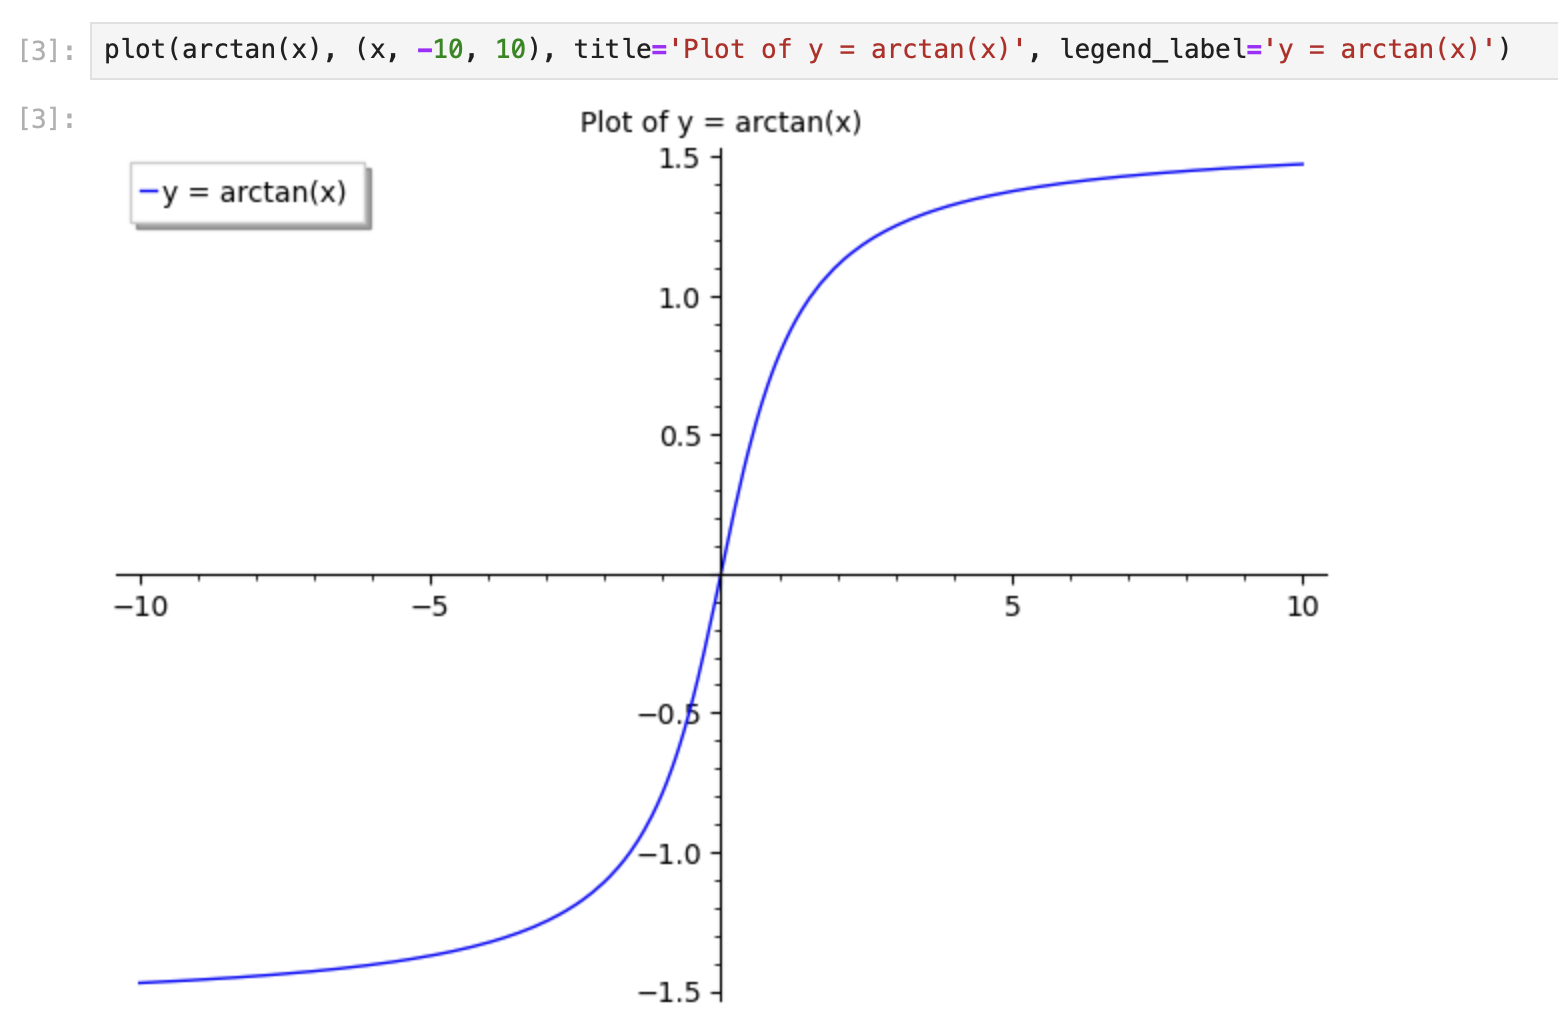
\includegraphics[height=8cm,width=15cm]{pdehw1}
   \end{minipage}
\end{center}
\end{proof}
\begin{theorem}
\begin{align}
\label{he2}
\text{ Solve }au_x+b u_y +cu=0
\end{align}
\end{theorem}
\begin{proof}
Fix 
\begin{align*}
\begin{cases}
  x'\triangleq ax+by \\
  y'\triangleq bx-ay
\end{cases}
\end{align*}
This map is clearly a diffeomorphism. Compute 
\begin{align*}
  \begin{cases}
    u_x= \frac{\partial u}{\partial x'}\frac{\partial x'}{\partial x}+\frac{\partial u}{\partial y'}\frac{\partial y'}{\partial x}=au_{x'}+bu_{y'}\\
    u_y=\frac{\partial u}{\partial x'}\frac{\partial x'}{\partial y}+\frac{\partial u}{\partial y'}\frac{\partial y'}{\partial y}=bu_{x'}-au_{y'}
  \end{cases}
\end{align*}
Plugging it back into the PDE in \myref{Equation}{he2}, we have 
\begin{align}
\label{he3}
cu+ (a^2+b^2)u_{x'}=0
\end{align}
If $c=a^2+b^2=0$, then all smooth functions are solution. If $a^2+b^2=0$ but $c\neq 0$, then clearly the only solution is $u=\tilde{0} $. If $a^2+b^2\neq 0$ but $c=0$, then $u_{x'}=\tilde{0}$, which implies $u=f(y')$ where $y'=bx-ay$ and  $f$ can be arbitrary smooth function.\\

Now, suppose $a^2+b^2\neq 0\neq c$, note that the PDE in \myref{Equation}{he3} is just an ODE of the form 
\begin{align*}
y+\frac{a^2+b^2}{c}y'=0
\end{align*}
The general solution to this ODE is 
\begin{align*}
y=Ce^{\frac{-ct}{a^2+b^2}}
\end{align*}
In other words, the general solution of the PDE in \myref{Equation}{he3} is 
\begin{align*}
u=C e^{\frac{-cx'}{a^2+b^2}}=Ce^{\frac{-c(ax+by)}{a^2+b^2}}
\end{align*}


\end{proof}
\section{HW2}
\begin{question}{}{}
Consider hear flow in a long circular cylinder where the temperature depends only on $t$ and on the distance $r$ to the axis of the cylinder. Here $r=\sqrt{x^2+y^2}$ is the cylindrical coordinate. From the three dimensional hear equation derive the equation $u_t=k (u_{rr}+\frac{u_r}{r})$
\end{question}
\begin{proof}
Write the three dimensional hear equation by 
\begin{align*}
u_t= k \Delta u
\end{align*}
Note that the Laplacian $\Delta u$ when written in cylindrical coordinate is 
\begin{align*}
\Delta u= u_{rr} + \frac{u_r}{r} +\frac{u_{\theta \theta}}{r^2} + u_{zz}
\end{align*}
Because the premise says that $u$ is constant in $z$ and  $\theta$, we know $u_{\theta \theta}=u_{zz}=0$
\begin{align*}
\Delta u = u_{rr}+ \frac{u_r}{r}
\end{align*}
This give us 
\begin{align*}
u_t= k (u_{rr}+ \frac{u_r}{r})
\end{align*}
\end{proof}
\section{1.2 First Order Linear Equations}
\begin{mdframed}
\textbf{(Principle of Geometric Method)} Given a first order homogeneous linear PDE with the form  
\begin{align*}
u_x+g(x,y)u_y=0
\end{align*}
We know if a curve $\gamma (x)= (x,y)$ satisfy 
\begin{align*}
\gamma '(x)= c_x(1,g(x,y))\text{ for some $c_x$ }
\end{align*} 
Then 
\begin{align*}
  (u\circ \gamma )'(x)=0\text{ for all $x$ }
\end{align*}
Since 
\begin{align*}
\gamma '(x)=(1, \frac{dy}{dx})
\end{align*}
To find $\gamma $, we only wish to solve 
\begin{align*}
\frac{dy}{dx}=g(x,y)
\end{align*}
\end{mdframed}
\begin{question}{}{}
Solve 
\begin{align*}
  (1+x^2)u_x+u_y=0
\end{align*}
\end{question}
\begin{proof}
The ODE 
\begin{align*}
\frac{dy}{dx}=\frac{1}{1+x^2}
\end{align*}
has general solution $y=\arctan x + C$, so 
\begin{align*}
u(x,y)=f(y-\arctan x)
\end{align*}
\end{proof}
\begin{question}{}{}
Solve 
\begin{align*}
\begin{cases}
  yu_x+xu_y=0\\
  u(0,y)=e^{-y^2}
\end{cases}
\end{align*}
In which region of the $xy$ plane is the solution uniquely determined? 
\end{question}
\begin{proof}
We are required to solve the ODE 
\begin{align*}
\frac{dy}{dx}= \frac{x}{y}
\end{align*}
Separating the variables and integrate 
\begin{align*}
\int yy' dx= \int xdx  \implies \frac{y^2}{2}= \frac{x^2}{2}+C
\end{align*}
This now implies 
\begin{align*}
u(x,y)=f(y^2-x^2)
\end{align*}
Initial Condition then give us 
\begin{align*}
u=e^{x^2-y^2}
\end{align*}

\end{proof}
\begin{question}{}{}
Solve the equation 
\begin{align*}
u_x+u_y=1
\end{align*}
\end{question}
\begin{proof}
Clearly $u=\frac{x}{2}+\frac{y}{2}$ is a solution. We now solve the PDE 
\begin{align*}
v_x+v_y=0
\end{align*}
Solving the ODE 
\begin{align*}
\frac{dy}{dx}=1
\end{align*}
we have 
\begin{align*}
y=x+C
\end{align*}
Thus the general solution is 
\begin{align*}
u=\frac{x}{2}+\frac{y}{2}+ f(y-x)
\end{align*}


\end{proof}
\begin{question}{}{}
Solve 
\begin{align*}
\begin{cases}
  u_x+u_y+u = e^{x+2y}\\
  u(x,0)=0
\end{cases}
\end{align*}
\end{question}
\begin{proof}
Let $\gamma (x)=x+C$, we have 
\begin{align*}
  (u\circ \gamma )'+(u\circ \gamma )= e^{3x+2C}
\end{align*}
We now solve the ODE 
\begin{align*}
y'+y=e^{3x+2C}
\end{align*}
The particular solution is clearly 
\begin{align*}
y=\frac{1}{4}e^{3x+2C}
\end{align*}
Thus the general solution is 
\begin{align*}
y=\frac{e^{3x+2C}}{4}+ \tilde{C}e^{-x} 
\end{align*}
We then now know 
\begin{align}
\label{uo}
  (u\circ \gamma )(x)= \frac{e^{3x+2C}}{4}+\tilde{C}e^{-x} 
\end{align}
In other words, 
\begin{align*}
u(x,x+C)= \frac{e^{3x+2C}}{4}+ \tilde{C}e^{-x} 
\end{align*}
Putting in the initial conditions, we have
\begin{align*}
0=u(-C,0)= \frac{e^{-C}}{4}+ \tilde{C}e^C 
\end{align*}
This implies 
\begin{align*}
\tilde{C}=\frac{-e^{-2C}}{4} 
\end{align*}
Putting the back into \myref{Equation}{uo}, we have 
\begin{align*}
u(x,x+C)= \frac{e^{3x+2C}- e^{-x-2C}}{4}
\end{align*}
So 
\begin{align*}
u(x,y)=\frac{e^{3x+2(y-x)}-e^{-x-2(y-x)}}{4}
\end{align*}
\end{proof}
\begin{question}{}{}
Use the coordinate method to solve the equation 
\begin{align*}
u_x+2u_y+(2x-y)u=2x^2 + 3xy -2y^2
\end{align*}
\end{question}
\begin{proof}
Let 
\begin{align*}
\begin{cases}
  \xi\triangleq 2x-y \\
  \eta  \triangleq x+2y 
\end{cases}
\end{align*}
We see 
\begin{align*}
\begin{cases}
  u_{\xi}=\frac{2}{5}u_x -\frac{1}{5}u_y\\
  u_{\eta }= \frac{1}{5}u_x + \frac{2}{5}u_y
\end{cases}
\end{align*}
We then can rewrite 
\begin{align}
\label{5ua}
5 u_\eta + \xi u= \xi \eta 
\end{align}
which clearly have particular solution 
\begin{align*}
u=\eta - \frac{5}{\xi} 
\end{align*}
To solve the linear homogeneous PDE 
\begin{align*}
5u_{\eta}+ \xi u =0
\end{align*}
Observe that for all fixed $\xi$, the PDE is just an ODE whose solution is exactly $u=C_\xi e^{\frac{-\xi \eta }{5}}$. We now know the general solution for \myref{PDE}{5ua} is exactly 
\begin{align*}
u=\eta - \frac{5}{\xi} +f(\xi) e^{\frac{-\xi \eta }{5}} 
\end{align*}
Then 
\begin{align*}
u= x+2y - \frac{5}{2x-y}+ e^{\frac{-(2x-y)(x+2y)}{5}} f(2x-y)
\end{align*}

\end{proof}
\section{1.4 Initial and Boundary Condition}
\begin{question}{}{}
Find a solution of 
\begin{align*}
\begin{cases}
  u_t=u_{xx}\\
  u(x,0)=x^2
\end{cases}
\end{align*}
\end{question}
\begin{proof}
Clearly $u=x^2+2t$ suffices.
\end{proof}
\section{1.5 Well Posed Problems}
\begin{question}{}{}
Consider the ODE
\begin{align*}
\begin{cases}
  u''+u=0\\
  u(0)=0\text{ and }u(L)=0
\end{cases} 
\end{align*}
Is the solution unique? Does the answer depend on $L$? 
\end{question}
\begin{proof}
We know the general solution space is exactly spanned by $\cos x$ and $\sin x$. Because 
\begin{enumerate}[label=(\alph*)]
  \item $u(0)=0$.
  \item $\sin 0=0$
  \item $\cos 0=1$
\end{enumerate}
we know the solution of our original ODE must be of the form 
\begin{align*}
u(x)=C \sin x
\end{align*}
This implies that the solution is unique if and only if $2\pi \not\equiv L$ (mod $2\pi$)
\end{proof}
\begin{question}{}{}
Consider the ODE 
\begin{align*}
\begin{cases}
  u''+u'=f \\
  u'(0)=u(0)=\frac{1}{2}(u'(l)+u(l))
\end{cases}
\end{align*}
where $f$ is given. 
\begin{enumerate}[label=(\alph*)]
  \item Is the solution unique? 
  \item Does a solution necessarily exist, or is there a condition that $f$ must satisfy for existence? 
\end{enumerate}
\end{question}
\begin{proof}
The solution space of linear homogeneous ODE $u''+u'=0$  is spanned by $e^{-x}$ and constant. If we add in the initial condition  $u'(0)=u(0)$, then the solution space become the subspace spanned by $e^{-x}-2$. One can check that if $u \in\operatorname{span}(e^{-x}-2)$, then 
\begin{align*}
u(0)=\frac{1}{2}(u'(l)+u(l))\text{ for all $l\inr$ }
\end{align*}
We now know the solution of the original ODE is not unique, since any solution added by $e^{-x}-2$ is again a solution. \\

Integrating both side on $[0,l]$, we see that given the boundary conditions, $f$ must satisfy 
\begin{align*}
\int_0^l f(x)dx=0
\end{align*}
\end{proof}
\begin{question}{}{}
Consider the Neumann problem 
\begin{align*}
\Delta u=f(x,y,z)\text{ in }D\text{ and } \frac{\partial u}{\partial n}=0\text{ on }\operatorname{bdy}D
\end{align*}
\begin{enumerate}[label=(\alph*)]
  \item What can we add to any solution to get another solution? 
  \item Use the divergence Theorem and the PDE to show that 
  \begin{align*}
  \iiint_D f(x,y,z)dxdydz=0
  \end{align*}
  is a necessary condition for the Neumann problem to have a solution. 
\end{enumerate}
\end{question}
\begin{proof}
Clearly, constants suffices, and observe 
\begin{align*}
\iiint_D fdxdydx=\iiint_D \Delta u dxdydz= \iiint_D \nabla \cdot (\nabla u)dxdydz = \iint_{\operatorname{bdy}D} \nabla u \cdot \textbf{n}dS= 0
\end{align*}
\end{proof}
\begin{question}{}{}
Consider the equation 
\begin{align*}
u_x+yu_y=0 
\end{align*}
with the boundary condition $u(x,0)=\phi (x)$. 
\begin{enumerate}[label=(\alph*)]
  \item $\phi (x)=x \implies $ no solution exists
  \item $\phi (x)=1 \implies $ multiple solutions exist.
\end{enumerate}
\end{question}
\begin{proof}
Using the geometric method, we see the characteristic curve is exactly $y=\tilde{C}e^x$. Thus the general solution is of the form 
\begin{align*}
u(x,y)=f(e^{-x}y)
\end{align*}
The boundary condition implies 
\begin{align*}
\phi (x)=u(x,0)=f(0)
\end{align*}
The result then follows. 
\end{proof}
\section{Types of Second-Order Equations} 
\begin{mdframed}
Consider the constant coefficient Linear PDE 
\begin{align*}
u_{xx}+2a_{12}u_{xy}+a_{22}u_{yy}+a_1u_x+a_2u_y+a_0u=0 
\end{align*}
Ignoring the term with order less than $2$, we have 
\begin{align*}
u_{xx}+2a_{12}u_{xy}+a_{22}u_{yy}=0 
\end{align*}
Or equivalently 
\begin{align*}
  (\partial_x + a_{12}\partial_y)^2 u + ( a_{22}-a_{12}^2)\partial_{yy} u =0 
\end{align*}
Now, if we set  
\begin{align*}
x\triangleq \xi \text{ and }y\triangleq a_{12}\xi + (\abso{a_{22}-a_{12}^2})^{\frac{1}{2}}\eta 
\end{align*}
we see that 
\begin{align*}
\begin{cases}
  a_{22}-a_{12}^2>0 \implies u_{\xi \xi}+u_{\eta \eta  }=0 \hspace{0.5cm}(\text{Elliptic})\\
  a_{22}-a_{12}^2=0 \implies u_{\xi \xi}=0\hspace{0.5cm}(\text{Parabolic})\\
  a_{22}-a_{12}^2 < 0 \implies u_{\xi \xi}-u_{\eta \eta  }=0\hspace{0.5cm}(\text{Hyperbolic})
\end{cases}
\end{align*}
More generally, if we are given 
\begin{align*}
a_{11}u_{xx}+2a_{12}u_{xy}+a_{22}u_{yy}=0
\end{align*}
then the discriminant is exactly 
\begin{align*}
a_{11}a_{22}-a_{12}^2
\end{align*}
\end{mdframed}
\begin{question}{}{}
What is the type of each of the following equations. 
\begin{enumerate}[label=(\alph*)]
  \item $u_{xx}-u_{xy}+u_{yy}+\cdots +u =0$. 
  \item $9u_{xx}+6u_{xy}+u_{yy}+u_x=0$
\end{enumerate}
\end{question}
\begin{question}{}{}
Find the regions in the $xy$ plane where the equation 
 \begin{align*}
   (1+x)u_{xx}+2xyu_{xy}-y^2u_{yy}=0
\end{align*}
is elliptic, hyperbolic, or parabolic. Sketch them. 
\end{question}
\begin{proof}
The discriminant is exactly 
\begin{align*}
  (xy)^2- (1+x)(-y^2)&=x^2y^2+xy^2+y^2\\
  &=y^2 (x^2+x+1)\\
  &=y^2[(x+\frac{1}{2})^2+ \frac{3}{4}]
\end{align*}
It then follows that the equation is parabolic if and only if $y=0$, and hyperbolic if and only if  $y\neq 0$. 

\end{proof}
\begin{question}{}{}
Reduce the elliptic equation 
\begin{align*}
u_{xx}+3u_{yy}-2u_x+24u_y+5u=0
\end{align*}
to the form 
\begin{align*}
v_{xx}+v_{yy}+cv=0
\end{align*}
by a change of dependent variable 
\begin{align*}
u\triangleq ve^{\alpha x+\beta  y}
\end{align*}
then a change of scale 
\begin{align*}
y'=\gamma y
\end{align*}
\end{question}
\begin{question}{}{}
Consider the equation $3u_y+u_{xy}=0$.
\begin{enumerate}[label=(\alph*)]
  \item What is its type? 
  \item Find the general solution. (Hint: Substitute $v=u_y$).
  \item With the auxiliary conditions $u(x,0)=e^{-3x}$ and $u_{y}(x,0)=0$, does a solution exist? Is it unique? 
\end{enumerate}
\end{question}
\section{PDE HW 3}
\begin{question}{}{}
Find a solution of 
\begin{align*}
\begin{cases}
  u_t=u_{xx}\\
  u(x,0)=x^2
\end{cases}
\end{align*}
\end{question}
\begin{proof}
Clearly $u=x^2+2t$ suffices.
\end{proof}
\begin{question}{}{}
Consider the ODE
\begin{align*}
\begin{cases}
  u''+u=0\\
  u(0)=0\text{ and }u(L)=0
\end{cases} 
\end{align*}
Is the solution unique? Does the answer depend on $L$? 
\end{question}
\begin{proof}
We know the general solution space is exactly spanned by $\cos x$ and $\sin x$. Because 
\begin{enumerate}[label=(\alph*)]
  \item $u(0)=0$.
  \item $\sin 0=0$
  \item $\cos 0=1$
\end{enumerate}
we know the solution of our original ODE must be of the form 
\begin{align*}
u(x)=C \sin x
\end{align*}
This implies that the solution is unique if and only if $2\pi \not\equiv L$ (mod $2\pi$)
\end{proof}
\begin{question}{}{}
Find the regions in the $xy$ plane where the equation 
 \begin{align*}
   (1+x)u_{xx}+2xyu_{xy}-y^2u_{yy}=0
\end{align*}
is elliptic, hyperbolic, or parabolic. Sketch them. 
\end{question}
\begin{proof}
The discriminant is exactly 
\begin{align*}
  (xy)^2- (1+x)(-y^2)&=x^2y^2+xy^2+y^2\\
  &=y^2 (x^2+x+1)\\
  &=y^2[(x+\frac{1}{2})^2+ \frac{3}{4}]
\end{align*}
It then follows that the equation is parabolic if and only if $y=0$, and hyperbolic if and only if  $y\neq 0$. 

\end{proof}
\chapter{Differential Geometry HW} 
\section{HW1} 
\begin{abstract}
In this HW, we give precise definition to $\P^n$  and $\RP^n$, and we rigorously show
\begin{enumerate}[label=(\alph*)]
  \item $\RP^n$  has a smooth structure. 
  \item $\P^n$ is homeomorphic to $\RP^n$ 
   \item $\P^n$ has a smooth structure.
\end{enumerate}
Note that in this PDF, brown text is always a clickable hyperlink reference. 
\end{abstract}
\begin{mdframed}
Define an equivalence relation on $\R^{n+1}\setminus \set{\textbf{0}}$ by 
\begin{align*}
\textbf{x}\sim \textbf{y}\overset{\triangle}{\iff }\textbf{y}=\ld \textbf{x}\text{ for some $\ld \inr^*$ } 
\end{align*}
Let $\RP ^n\triangleq (\R^{n+1}\setminus \set{\textbf{0}})\setminus \sim $ be the quotient space and let  
\begin{align*}
V_i\triangleq \set{\textbf{x}\inr^{n+1}:\textbf{x}^i \neq 0}\text{ for each }1\leq i\leq n+1
\end{align*}
By definition, it is clear that 
\begin{align*}
\text{ either }\pi^{-1}(\pi (\textbf{x}))\subseteq V_i\text{ or }\pi^{-1}(\pi (\textbf{x}))\subseteq V_i^c
\end{align*}
Then if we define $\phi_i:V_i\rightarrow \R^n$ by
\begin{align*}
\phi_i(\textbf{x})\triangleq \Big(\frac{\textbf{x}^1}{\textbf{x}^i},\dots ,\frac{\textbf{x}^{i-1}}{\textbf{x}^i},\frac{\textbf{x}^{i+1}}{\textbf{x}^i},\dots,\frac{\textbf{x}^{n+1}}{\textbf{x}^i} \Big)
\end{align*}
because $\pi (\textbf{x})=\pi(\textbf{y})\implies \phi_i(\textbf{x})=\phi_i(\textbf{y})$, we can well induce a map 
\begin{align*}
\Phi_i:U_i\triangleq \pi (V_i)\subseteq \R P^n\rightarrow \R^n; \pi (\textbf{x})\mapsto \phi_i(\textbf{x})
\end{align*}
Note that one has the equation 
\begin{align*}
\Phi_i(\pi (\textbf{x}))= \phi_i(\textbf{x})\text{ for all }\textbf{x}\in V_i
\end{align*}
\end{mdframed}
\begin{theorem}
\textbf{(Real Projective Space with a differentiable atlas)} We have
\begin{align*}
  \R P^n\text{ with atlas }\set{(U_i,\Phi_i):1\leq i\leq n+1}\text{ is a differentiable manifold }
\end{align*}
\end{theorem}
\begin{proof}
We are required to prove 
\begin{enumerate}[label=(\alph*)] 
  \item $(U_i,\Phi_i)$ are all charts. 
  \item $\set{(U_i,\Phi_i):1\leq i\leq n+1}$ form a differentiable atlas. 
\item $\R P^n$ is Hausdorff.
\item $\R P^n$ is second-countable. 
\end{enumerate}
 Because $\pi^{-1}(U_i)=V_i$ and $V_i$ is clearly open in $\R^{n+1}\setminus \set{\textbf{0}}$, we know $U_i\subseteq \R P^n$ is open. Note that clearly,   $\Phi_i(U_i)=\R^n$. To show $(U_i,\Phi_i)$ is a chart, it remains to show that $\Phi_i$ is a homeomorphism between $U_i$ and  $\R^n$.  It is straightforward to check $\Phi_i$ is one-to-one on $U_i$. This implies $\Phi_i$ is a bijective between $U_i$ and  $\R^n$. \\


Fix open $E\subseteq \R^n$. We see 
\begin{align*}
  \pi^{-1}(\Phi_i^{-1}(E))=\phi_i^{-1}(E)
\end{align*}
Then because $\phi_i:V_i\rightarrow \R^n$ is clearly continuous, we see $\phi_i^{-1}(E)$ is open in $\R^{n+1}\setminus \set{\textbf{0}}$, and it follows from definition of quotient topology  $\Phi_i^{-1}(E)\subseteq \R P^n$ is open. Then because $U_i$ is open in  $\R P^n$, we see $\Phi_i^{-1}(E)$ is open in $U_i$. We have proved  $\Phi_i:U_i\rightarrow \R^n$ is continuous.\\


Define $\Psi_i: \R^n\rightarrow V_i$ by 
\begin{align*}
\Psi (\textbf{x}^1,\dots ,\textbf{x}^n)= (\textbf{x}^1,\dots ,\textbf{x}^{i-1},1,\textbf{x}^i,\dots ,\textbf{x}^n)
\end{align*}



Observe that for all $\textbf{x}\in \Phi_i(U_i)$, we have
\begin{align*}
\Phi_i^{-1}(\textbf{x})= \pi(\Psi_i (\textbf{x}))
\end{align*}
It then follows from $\Psi_i:\R^n\rightarrow V_i$ and $\pi:\R^{n+1}\setminus \set{\textbf{0}}\rightarrow \R P^n$ are continuous that $\Phi_i^{-1}:\R^n\rightarrow \R P^n$ is continuous.\\

We have proved that $(\Psi_i,U_i)$ are all charts. Now, because $V_i$ clearly cover $\R^{n+1}$, we know $U_i$ also cover  $\R P^n$. We have proved $\set{(U_i,\Phi):1\leq i\leq n+1}$ form an atlas. The fact $\R P^n$ is second-countable follows. \\

Fix $(\textbf{x}_1,\dots ,\textbf{x}_{n})\in \Phi_i(U_i\cap U_j)$. We compute 
\begin{align*}
\Phi_j\circ \Phi_i^{-1} (\textbf{x}^1,\dots ,\textbf{x}^{n} )&=\Phi_j \Big( [(\textbf{x}^1,\dots ,\textbf{x}^{i-1},1,\textbf{x}^i,\textbf{x}^{i+1},\dots, \textbf{x}^n)] \Big) \\
&= \begin{cases}
  (\frac{\textbf{x}^1}{\textbf{x}^j},\dots , \frac{\textbf{x}^{j-1}}{\textbf{x}^j},\frac{\textbf{x}^{j+1}}{\textbf{x}^j},\dots ,\frac{\textbf{x}^{i-1}}{\textbf{x}^j},\frac{1}{\textbf{x}^j},\frac{\textbf{x}^i}{\textbf{x}^j},\dots ,\frac{\textbf{x}^n}{\textbf{x}^j})& \text{ if $j<i$ }\\
  (\frac{\textbf{x}^1}{\textbf{x}^{j-1}},\dots , \frac{\textbf{x}^{i-1}}{\textbf{x}^{j-1}},\frac{1}{\textbf{x}^{j-1}},\frac{\textbf{x}^i}{\textbf{x}^{j-1}},\dots , \frac{\textbf{x}^{j-2}}{\textbf{x}^{j-1}}, \frac{\textbf{x}^j}{\textbf{x}^{j-1}}, \dots,\frac{\textbf{x}^n}{\textbf{x}^{j-1}})& \text{ if $j>i$ }
\end{cases}
\end{align*}
This implies our atlas is indeed differentiable. \\

Before we prove $\RP^n$ is Hausdorff, we first prove that  \olive{$\pi:\R^{n+1}\setminus \set{\textbf{0}}\rightarrow \RP^n$ is an open mapping}. Let $U\subseteq \R^{n+1}\setminus \set{\textbf{0}}$ be open. Observe that 
\begin{align*}
\pi^{-1}(\pi(U))= \set{t\textbf{x}\inr^{n+1}:t\neq 0\text{ and }\textbf{x}\in U}
\end{align*}
Fix $t_0\textbf{x}\in \pi^{-1}(\pi (U))$. Let $B_\epsilon (\textbf{x})\subseteq U$. Observe that
\begin{align*}
B_{\abso{t_0}\epsilon }(t_0\textbf{x})\subseteq t_0B_\epsilon (\textbf{x})\subseteq t_0U\subseteq \pi^{-1}(\pi (U))
\end{align*}
This implies $\pi ^{-1}(\pi (U))$ is open.  $\odone$ \\

Now, \customref{Hausdorff and Quotient}{because $\pi$ is open, to show $\RP^n$ is Hausdorff, we only have to show}
 \begin{align*}
R_\pi \triangleq \set{(\textbf{x},\textbf{y})\in (\R^{n+1}\setminus \set{\textbf{0}})^2:\pi (\textbf{x})= \pi (\textbf{y})}\text{ is closed }
\end{align*}
Define $f:(\R^{n+1}\setminus \set{\textbf{0}})^2\rightarrow \R$ by 
\begin{align*}
f(\textbf{x},\textbf{y})\triangleq \sum_{i\neq j} (\textbf{x}^i\textbf{y}^j-\textbf{x}^j \textbf{y}^i)^2
\end{align*}
Note that $f$ is clearly continuous and $f^{-1}(0)=R_\pi$, which finish the proof.
\end{proof}
\begin{mdframed}
Alternatively, we can characterize $\R P^n$ by identifying the antipodal pints on $S^n\triangleq \set{\textbf{x}\inr^{n+1}:\abso{\textbf{x}}=1}$ as one point 
\begin{align*}
\textbf{x}\sim \textbf{y}\overset{\triangle}{\iff } \textbf{x}=\textbf{y}\text{ or }\textbf{x}=-\textbf{y}
\end{align*}
and let $\P^n\triangleq S^n\setminus \sim $ be the quotient space.
\end{mdframed}
\begin{theorem}
\label{RPnhom}
\textbf{(Equivalent Definitions of Real Projective Space)} 
\begin{align*}
\RP^n\text{ and }\P^n\text{ are homeomorphic }
\end{align*}
\end{theorem}
\begin{proof}
Define $F:\P^n\rightarrow \RP^n$ by 
\begin{align*}
\set{\textbf{x},-\textbf{x}}\mapsto \set{\ld  \textbf{x}:\ld \inr^*}
\end{align*}
It is straightforward to check that $F$ is well-defined and bijective. Define $f:S^n \rightarrow \R P^n$ by 
\begin{align*}
f= \pi \circ \textbf{id}
\end{align*}
where $\textbf{id}:S^n \rightarrow \R^{n+1}\setminus \set{\textbf{0}}$ and $\pi:\R^{n+1}\setminus \set{\textbf{0}}\rightarrow \R P^n$ are continuous. Check that  
\begin{align*}
f=F\circ p
\end{align*}
where $p:S^n\rightarrow \P^n$ is the quotient mapping. It now follows from the \customref{quotient property}{universal property} that $F$ is continuous, and since $\P^n$ is compact and  $\R P^n$ is Hausdorff,  it also follows that  \customref{HbC}{$F$ is a homeomorphism between $\R P^n$ and  $\P^n$}. 
\end{proof}
\begin{mdframed}
Knowing that $F:\P^n\rightarrow \RP^n$ is a homeomorphism and $\RP^n$ is a smooth manifold, we see that  $\P^n$ is Hausdorff and second-countable, and if we define the atlas 
\begin{align*}
  \set{(F^{-1}(U_i), \Phi_i \circ F):1\leq i\leq n+1}
\end{align*}
We see this atlas is indeed smooth, since 
\begin{align*}
  (\Phi_i\circ F)\circ (\Phi_j \circ F)^{-1}=\Phi_i \circ \Phi_j^{-1}
\end{align*}
\end{mdframed}

\section{Appendix}
\begin{theorem}
\label{HbC}
\textbf{(Homeomorphism between Compact Space and Hausdorff Space)} Suppose 
\begin{enumerate}[label=(\alph*)]
  \item $X$ is compact.  
  \item $Y$ is Hausdorff.  
  \item $f:X\rightarrow Y$ is a continuous bijective function. 
\end{enumerate}
Then 
\begin{align*}
f\text{ is a homeomorphism between }X\text{ and }Y
\end{align*}
\end{theorem}
\begin{proof}
Because closed subset of compact set is compact and continuous function send compact set to compact set, we see for each closed $E\subseteq X$, $f(E)\subseteq Y$ is compact. The result then follows from \customref{Compact Subspace of Hausdorff Space is Closed}{$f(E)\subseteq Y$ being closed since $Y$ is Hausdorff}. 
\end{proof}
\begin{theorem}
\label{Hausdorff and Quotient}
  \textbf{(Hausdorff and Quotient)} If $\pi:X\rightarrow Y$ is an open mapping, and we define
\begin{align*}
R_\pi\triangleq \set{(x,y)\in X^2 : \pi (x)=\pi (y)} 
\end{align*}
Then
\begin{align*}
R_\pi\text{ is closed }\iff Y\text{ is Hausdorff }
\end{align*}
\end{theorem}
\begin{proof}
  Suppose $R_\pi$ is closed. Fix some $x,y$ such that $\pi (x)\neq \pi (y)$. Because $R_\pi$ is closed, we know there exists open neighborhood $U_x,U_y$ such that $U_x \times U_y \subseteq (R_\pi)^c$. It is clear that $\pi (U_x),\pi (U_y)$ are respectively open neighborhood of $\pi (x)$ and $\pi (y)$. To see $\pi (U_x)$ and $\pi (U_y)$ are disjoint, \red{assume} that $\pi (a)\in \pi (U_x)\cap \pi (U_y)$. Let $a_x\in U_x$ and $a_y\in U_y$ satisfy $\pi (a_x)=\pi (a)=\pi (a_y)$, which is impossible because $(a_x,a_y)\in (R_\pi)^c$. \CaC\\


Suppose $Y$ is Hausdorff. Fix some  $x,y$ such that  $\pi (x)\neq \pi (y)$. Let $U_x,U_y$ be open neighborhoods of  $\pi (x),\pi (y)$ separating them. Observe that $(x,y)\in \pi^{-1}(U_x)\times \pi^{-1}(U_y)\subseteq (R_\pi)^c$
\end{proof}

\section{Example: $S^1,\R\setminus \Z$ diffeomorphism } 
\begin{mdframed}
Equip $S^1\triangleq \set{(x,y)\inr^2: \abso{(x,y)}=1}$ with the standard four projection chart smooth atlas  as one of them being
\begin{align*}
V\triangleq  \set{(x,y)\inr^2: y>0}\text{ and }\phi_V: V\rightarrow \R; (x,y)\mapsto  x
\end{align*}
Let $p:\R\rightarrow \R\setminus \Z$  be the quotient map and let 
\begin{align*}
U_0\triangleq p\Big((0,1)\Big)\text{ and }U_1\triangleq p\Big((\frac{-1}{2},\frac{1}{2})\Big)
\end{align*}
which are both open as one can readily check. Define $\phi_0:U_0\rightarrow (0,1)$ by 
\begin{align*}
\phi_0 (p(t))\triangleq t_0\text{ where $t_0\in (0,1)$ and $p(t_0)=p(t)$ }
\end{align*}
and $\phi_1:U_1\rightarrow (-\frac{1}{2},\frac{1}{2})$ by
\begin{align*}
\phi_1(p(t))\triangleq t_0\text{ where }t_0 \in (-\frac{1}{2},\frac{1}{2})\text{ and }p(t_0)=p(t)
\end{align*}
Clearly, the function $G:\R\setminus \Z\rightarrow S^1$ well-defined by $G(p(x))\triangleq (\cos 2\pi x, \sin 2\pi x)$ is a homeomorphism, as one can check that 
\begin{enumerate}[label=(\alph*)]
  \item $G$ is a continuous bijection. (Using Universal property of quotient map)
  \item $\R\setminus \Z$ is compact. (by finite sub-cover definition)
  \item $S^1$ is Hausdorff.
\end{enumerate}
We now compute that $\phi_V\circ G\circ \phi_0^{-1}$ is defined on whole $(0,1)$, and is exactly 
\begin{align*}
\phi_V\circ G\circ \phi_0^{-1}(t)\triangleq \cos 2\pi t\text{ smooth }
\end{align*}
\end{mdframed}
\end{document}
